%
% This edited using www.sharelatex.com
%
\documentclass[5p]{elsarticle} % use the 5p option to see in two column, use the preprint option for how they want to see it when we submit it to them

\usepackage{url}
\usepackage{amsmath}
\usepackage{amssymb}
\usepackage{hyperref}

\newcommand{\orcid}[1]{\href{https://orcid.org/#1}{\includegraphics[width=8pt]{orcid.png}}}

\journal{International Journal of Hydrogen Energy}

% This next bit patches the Elsevier ``Preprint submitted to.." footer
% on the first page
\makeatletter
\def\ps@pprintTitle{%
    \let\@oddhead\@empty
    \let\@evenhead\@empty
    \def\@oddfoot{\centerline{\hspace*{\fill} \raggedright DRAFT: \today} }%
    \let\@evenfoot\@oddfoot}
\makeatother
     
\begin{document}
\begin{frontmatter}

% This bit is needed to let elsarticle-num-names format doi links properly 
\makeatletter
\providecommand{\doi}[1]{%
  \begingroup
    \let\bibinfo\@secondoftwo
    \urlstyle{rm}%
    \href{http://dx.doi.org/#1}{%
      doi:\discretionary{}{}{}%
      \nolinkurl{#1}%
    }%
  \endgroup
}
\makeatother
\bibliographystyle{elsarticle-num} % doesn't allow citet, but does format doi properly

\hyphenation{pipe-work}

\title{Moving Hydrogen through the UK Gas Distribution Network}


\author[mjs]{Michael Sargent  \orcid{0000-0001-9129-2990}\corref{cor1} }
\ead [mjs] {0000-0001-9129-2990}
\ead{michael.sargent@cambridgeenergy.uk}

\author[mjs]{Philip Sargent  \orcid{0000-0002-1825-0097}}
\ead [pms] {0000-0002-0968-4467}
\ead{philip.sargent@cambridgeenergy.uk}

% \includegraphics[width=8pt]{orcid.png}
\cortext[cor1]{Corresponding author: Michael Sargent}

  \address[mjs]{Cambridge Energy UK, 27 Greville Road, Cambridge CB1 3QJ, UK }
 
  
\newcommand{\sshratio}{3.292} % just the \textsc{hhv} ratio
\newcommand{\ssvratio}{3.076} % velocity ratio
\newcommand{\sspratio}{1.294} % pressure ratio
\newcommand{\sseratio}{3.980}  % energy ratio

\begin{abstract}

We state the appropriate thermodynamic and transport properties to use for the delivery of hydrogen through pre-existing natural gas distribution networks. We show that the flow is not as fully-turbulent as past work has assumed, that hydrogen makes the flow even less turbulent, and that the pipe friction calculation requires more careful treatment in this partially-turbulent regime.

We propose that the relevant final energy demand is the  energy delivered as heated water. The different dew points of the flue gases from hydrogen versus natural gas combustion affect the boiler efficiency. This impacts the relative amount of hydrogen required to be delivered.

We find that to deliver the same amount of useful energy as hot water, hydrogen requires a gas velocity of 3.076$\times$ and a pressure gradient that is \sspratio$\times$  higher. The compression power increase required to deliver hydrogen through the low pressure network can be up to 7.8$\times$  that for natural gas.

\end{abstract}

% maximum of 6 keywords, using American spelling
\begin{keyword}
Hydrogen\sep pipe-flow\sep  friction factor\sep  natural gas\sep condensing boiler\sep gas velocity.
\end{keyword}

\end{frontmatter}

\section{Introduction}

A possible future for the UK gas network is to reuse parts of it to distribute hydrogen instead of natural gas\citep{dodds2013}. Two recent reports\citep{RoyalAcademyofEngineering2022, ARUP2023} excellently summarise the current complex issues regarding replacing natural gas with hydrogen in the UK in political and techno-economic terms, however they do not cover the detailed flow characteristics of hydrogen in pipes.

In recent years it has become apparent that reusing parts of the low pressure distribution grid is a very different problem from re-using the the intermediate pressure distribution grid or the transmission grid\citep{H2Blends21,natgas2023}.

While a high pressure transmission system for hydrogen may be required in the UK\citep{Samsatli2019}, this would largely be new construction built in parallel with the existing natural gas National Transmission System. However parts of the intermediate and low pressure distribution system would be repurposed from natural gas to carry hydrogen. 

We have determined that there are no prior, sound, theory-based studies of thr flow of hydrogen through pipes under the conditions typical of the last sections of the distribution network.

Therefore, these are the questions we want to answer:
\begin{enumerate}
\item Can the pipework supply enough hydrogen to match the energy demand of domestic housing?
\item What are the pressure and gas velocity differences?
\item How much extra energy would be required to deliver the hydrogen?
\end{enumerate}

\subsection{Bossel}

The first attempt at 
%these calculations 
this work 
was made by Bossel\citep{bossel2006} but he considered pure methane, not natural gas, through a transmission pipe with assumed fully-turbulent flow. To date, Bossel is still used\citep{Ibrahim2022} as a basis flow calculations, even for situations outside his original assumptions, and full reassessment of his first-principles calculation is overdue.

In the distribution system we find that non-linear friction effects become significant and the flow is not fully-turbulent. Models which have used Bossel's number are  inaccurate for distribution and may not be quite right for transmission either, quite apart from using the wrong gas.

\subsection{Out of scope}

Distributing hydrogen has other complexities that this paper does not address. 
These include 
maintaining the required concentration when blended with natural gas\citep{H2Blends21}, 
Joule-Thompson cooling and liquid dropout\citep{Schouten2004}, 
compressor issues\citep{Wit2018}, 
compatibility with vehicle tanks\citep{Altfeld2013}, 
linepack and high- and intermediate pressure networks\citep{Witek2022}, 
and
materials issues\citep{ARUP2023}.

\section{Standard gas and reference conditions}
\label{sec:standards}

Public data on the exact composition of natural gas in the UK national transmission system is sparse.
%, as the gas is a mixture of different gas fields that are processed together, and the composition %changes over time and varies across the network
There are regulatory limits on certain properties of the gas, including the Wobbe  
%(see \ref{sec:wobbe}
number, density, and calorific value under defined conditions.

\begin{table}[htb]
    \centering
    \begin{tabular}{r|r|r|r}
        & [mol/mol]  && [mol/mol]\\
        \hline
        CH$_4$    & 89.5514  \% & iC$_5$    &  0.0344 \%\\
        C$_2$H$_6$   &  5.1196  \% & neoC$_5$  &  0.0020 \%\\
        C$_3$H$_8$   &  1.3549  \% & C$_6$     &  0.2377 \%\\
        nC$_4$    &  0.2162  \% & CO$_2$    &  2.0743 \%\\
        iC$_4$    &  0.1269  \% &N$_2$     &  0.9354 \%\\
        nC$_5$    &  0.3472  \% &   &  \\
         \hline
    \end{tabular}
    \caption{Composition of NG at Fordoun NTS on 20th Jan.2021.\citep{cngservices2019}}
    \label{tab:Fordoun}
\end{table}

As a concrete example, this paper uses the composition of the gas taken directly from an 84~bar NTS transmission pipe at Fordoun (near Aberdeen) on 20 Jan.2021\citep{cngservices2019} as the composition of natural gas (NG). 

This gas has  11 components: methane, ethane, propane, n-butane, iso-butane, n-pentane, iso-pentane, neo-pentane, hexane (including traces of higher hydrocarbons), carbon dioxide, and nitrogen. 
The Peng-Robinson equation of state can be used to calculate the average properties
% (see \ref{sec:gasmix})
of this mixture\citep{Sargents_github}. 
The mixture has a molecular weight of 18.359~g/mol, a higher heating value of 940.813~kJ/mol and a density of 0.83556~kg/m$^3$ at 8$^\circ$C.

The conditions of the gas in the distribution network that were used for these and all other material properties are representative of gas in the Service Line pipe entering a UK home during winter. 
The temperature of the gas in the distribution network is not significantly different from that of the surrounding ground, and the ground temperature at the depth of the distribution network will be about $8^\circ$C during the winter months  on average\citep{MacKay2008}.
The average pressure in the distribution network is taken to be 40~mbar above one atmosphere (1.05325 bar)\citep{ARUP2023,utonomy23}\footnote{We do not consider deviations from these conditions for the purpose of calculating material parameters, as the deviations in conditions are not large enough to cause significant changes to the material parameters}.

\section{Delivering combustion energy through a pipe}
\label{sec:pipe}

In comparing the delivery of natural gas and hydrogen through a pipe system, the metric by which they must be evaluated is the delivery of the same heat to the consumer. 

\subsection{Molar Properties}
\label{sec:molar}

When dealing with natural gas, quantities of the gas are often expressed either as mass, or volume at standard temperature and pressure. 
However as we are comparing different compressible gases (see \ref{appendix:gasprops}), both in the transport as well as the chemical reaction of combustion, we shall work in moles of gas.
An ideal gas obeys the ideal gas law, equation \eqref{eqn:ideal}.

\begin{equation}
    \label{eqn:ideal}
    P \: V_{ideal} = n \: R \: T
\end{equation}
where $n$ is the number of moles of gas, $R$ is the ideal gas constant (8.3145 J/mol$\cdot$K), $P$ is the absolute pressure, and $T$ is the absolute temperature.

We account for non-ideality of the gases by using the compressibility factor, $Z$, which is the ratio of the actual volume to that of an ideal gas under the same conditions:

\begin{equation}
    \label{eqn:compressiblity}
    Z = \frac{V_{real}}{V_{ideal}}
\end{equation}

$Z$ is related to the external conditions via the molar volume, the volume of one mole of gas, $V_m$, which is linearly proportional to $Z$ by the conditions of the gas:

\begin{equation}
    \label{eqn:molarvol}
    V_m = \frac{V_{real}}{n} = \frac{Z \: R \: T}{P}
\end{equation}

\subsection{Energy delivered}
\label{sec:energydelivered}

For the flow of a fuel through a pipe, such as the distribution system which supplies natural gas to domestic homes, the energy supply may be calculated by equation~\eqref{eqn:energysupply}.

\begin{equation}
\label{eqn:energysupply}
    Q = A \: v \: \frac{\textsc{[\textsc{hhv}]}}{V_m} \: \eta
    = A \: v \: \textsc{[\textsc{hhv}]} \: \frac{P}{Z \: R \: T} \: \eta
\end{equation}

$Q$, is the rate at which useful combustive energy is transferred along the pipe, in kJ/s. 
$A$ is the cross section area of the supply pipe in m$^2$.
$v$ is the linear velocity of the gas in m/s, which is the parameter that may be controlled to modify the rate of energy transfer to account for differences between the two gases. 

The  important gas properties are the molar volume, $V_m$, in m$^3$/mol, and the Higher Heating Value, $\textsc{[\textsc{hhv}]}$, also called the heat of combustion, in kJ/mol. 
Lastly, $\eta$ is the efficiency of combustion reactions of the gases within domestic boiler systems. 

To calculate the difference in gas velocity required for hydrogen compared to natural gas,   equation~\eqref{eqn:energysupply} is  calculated
for each gas\footnote{
The thermophysical data used in the paper come from NIST\citep{Huber2022} and also from the CoolProp project\citep{coolprop} which publishes the algorithms as open source code.}
for the same value of $Q$, and then the ratio of the two gives equation~\eqref{eqn:velocityratio}. 
We are considering the two gases in the same section of the distribution system, thus the pipe cross section area $A$ and the temperature $T$, which should be equal to the ground temperature, are not included as they will be the same for both gases.

\begin{equation}
\label{eqn:velocityratio}
    \left(\frac{v_{H_2}}{v_{NG}}\right) = 
    \frac{
        \left(\frac{Z_{H_2}}{Z_{NG}}\right) 
    }{
        \left(\frac{\textsc{[\textsc{hhv}]}_{H_2}}{\textsc{[\textsc{hhv}]}_{NG}}\right)  
        \left(\frac{P_{av,H_2}}{P_{av,NG}}\right)
        \left(\frac{\eta_{H_2}}{\eta_{NG}}\right)
    }
\end{equation}

Equation~\eqref{eqn:velocityratio} shows that there are four terms that affect how much more gas is needed when switching from natural gas to hydrogen, each given as a ratio: 
\begin{enumerate}
    \item Compressibility factors
    \item Higher heating values (by mole)
    \item Pipeline pressures (average)
    \item Boiler efficiencies
\end{enumerate}
We will look at 
%each of 
these ratios and compare the relative magnitudes of their effects on the overall velocity ratio.
Note that as this form uses the molar HHV, the effect of density has been confined to the compressibility factor.

\subsection{Compressibility factor}
\label{sec:compressibility}

The compressibility factor, $Z$, of any gas is a quantitative measure of its non-ideal behaviour. 
The temperature dependence of $Z$ for hydrogen, natural gas, and pure methane is shown in Figure~\ref{fig:peng_z}.
The dependence on pressure is very slight for the narrow pressure range present in the distribution system\citep{GS(M)2023, dodds2013}.

\begin{figure}[htbp]
\centering
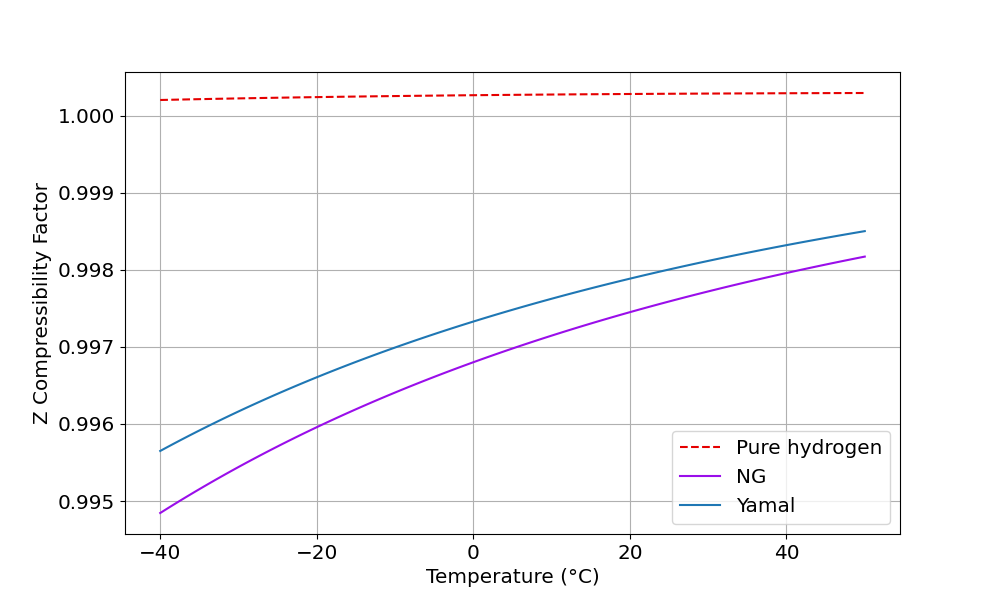
\includegraphics[width=0.48\textwidth]{peng_z.png}
\caption{Plot of gas compressibility factors $Z$, showing the deviation from the ideal gas value of 1.0 calculated using the Peng-Robinson equation of state at 8$^\circ$C\citep{Sargents_github}. The effect of 75~mbar pressure on Z is minute.}
\label{fig:peng_z}
\end{figure}

In the distribution pipework the compressibility factor of hydrogen is nearly constant at 1.0003 and the compressibility factor of natural gas is 0.997 at 8$^\circ$C\citep{Sargents_github}.  
This means that the ratio of compressibility factors is $Z_{H_2} / Z_{NG} = 1.003$.
This is a very small effect that is potentially within the uncertainty of other parameters in equation~\eqref{eqn:velocityratio}.

\subsection{Higher Heating Values \textsc{[\textsc{hhv}]}}
\label{sec:hhv}

Of these four terms in Equation~\eqref{eqn:velocityratio}, the \textsc{hhv} of the gases is the simplest as it is a molecular property that does not depend on the conditions of the gas.
All Higher Heating Value data are by convention referred to a standard temperature and pressure of 25$^\circ$C and 1~atm, i.e. close to room temperature.
The \textsc{hhv} is the energy of the reaction in which the fuel and oxygen start at 25$^\circ$C and 1~atm, are combusted, and then the sensible and latent heat of the combustion products is recovered as they are brought back down to 25$^\circ$C and all the water is condensed\citep{nist_delta_H}. 
The \textsc{hhv} of natural gas and hydrogen are shown in Table~\ref{tab:combust}.

\begin{table}[ht]
\centering
\begin{tabular}{l|c}
    & \textsc{hhv} [kJ/mol]\\
    \hline
    H$_2$ & 285.826 \\
    NG & 940.813 \\
    \hline
    ratio & 0.304  \\
    reciprocal & 3.292 \\
\end{tabular}
\caption{\label{tab:combust}Higher Heating Values at 25$^\circ$C and 1~atm.} 
\end{table}

A naive approximation to calculating the ratio of gas velocities may be made by assuming both gases to be close to ideal, the pressures close to atmospheric, and the boiler efficiencies to be the same for hydrogen and natural gas.
Under these assumptions, then the velocity ratio would be equal to the reciprocal of the \textsc{hhv} ratio as shown in Table~\ref{tab:combust}, and the velocity of hydrogen required to supply the same quantity of  heat would be 3.292~$\times$  that of natural gas. 
Previous studies have published a value of 3.13 for this velocity ratio, because they did not use the correct values for natural gas\citep{dodds2013,bossel2006}. 
The major cause of this difference is the approximately 7\% by mole of longer hydrocarbons in UK natural gas that raise the molar \textsc{hhv} significantly compared to pure methane (Table~\ref{tab:Fordoun}).

\subsection{Average pressure}
\label{sec:avpressure}

The average pressure in the distribution network will depend on the pressure drop in the delivery of the gas along the pipes, which in turn depends on the velocity of the gas.
We are using the average pressure for natural gas as 40~mbar above atmospheric\citep{utonomy23}, but we require a value for hydrogen. 
This requires an iterative solution procedure which will be performed in Section~\ref{sec:pressuredrop}, so for now we simply state the result, that the average pressure for hydrogen is 45.88~mbar above atmospheric.
Therefore the ratio of average pressures is ${P_{av,H_2}}/{P_{av,NG}} = 1.0056$.

\subsection{Boiler efficiency}
\label{sec:efficiency}

The efficiency of a domestic boiler is highly dependent on the design and operation of each individual unit. 
Rather than attempt to quantify the diverse array of domestic boilers  in use in the UK, we will instead look at how the \emph{maximum possible efficiency} differs for hydrogen and natural gas, and assume that the operation relative to this maximum efficiency is comparable for the two fuels.
This means we are not considering gas velocity or heat transfer within the heat exchanger section of the boiler.
We categorise boilers into one of two 
%different 
operating modes:

\begin{itemize}
    \item A non-condensing boiler vents the flue gas, the products of the combustion, with all of the water still in the gas phase.
    \item A condensing boiler attempts to recover latent heat by condensing some of the water vapour into liquid water. 
\end{itemize}

The \textsc{hhv} is the absolute maximum energy that may be obtained from the fuel
%, when combusted under the conditions mentioned in Section~\ref{sec:hhv}, 
so the boiler efficiency $\eta$ will be relative to the \textsc{hhv}\citep{saty2018}.
Furthermore, as the fuel is not burned in pure oxygen, there is sensible heat lost to heating up the nitrogen in the air. 
Also a  boiler will typically operate with 15\% excess air, to ensure complete combustion of the fuel\citep{CleaverBooks2016}.
Any heat which is not recovered by not condensing water vapour, and inlet and outlet gases not being at 25$^\circ$C and 1~atm, is a reduction in efficiency\citep{saty2018}.

\begin{multline}
    \label{eqn:NTSgreaction}
    [0.970 C_{1.119} H_{4.239} + 0.021 C O_2 + 0.0094 N_2] + 2.114 O_2 \longrightarrow \\
    1.106 C O_2 + 2.056 H_2 O + 0.0094 N_2
\end{multline}

The overall combustion reaction of one mole of the UK natural gas is given by equation~\eqref{eqn:NTSgreaction}, and the \textsc{hhv} of this reaction is 940.813~kJ/mol\citep{nist_delta_H}.
The list of reagents (fuel and air) and products of the combustion are shown in table~\ref{tab:NTSgcombustion}.
All of the combustible hydrocarbons have been combined into one pseudo-component\citep{coolprop} (see \ref{appendix:gasprops}), with a mole-averaged heat capacity of 37.276~kJ/mol$\cdot$K\citep{Huber2022} and the air is approximated as a mixture of 20.95\% oxygen and 79.05\% nitrogen\footnote{The weather-dependent humidity of the inlet air has an insignificant effect on the subsequent calculations, as does the small quantity of the pollutant $NO_{x}$ produced in the combustion.}

\begin{small}
\begin{table}[ht]
    \centering
    \begin{tabular}{r|ccc|l}
         Species & Reagents & Products & Products & C$_p$ \\
         & {\small[mol]} & {\small[mol]} & {\small[mol/mol]} & {\small[J/mol$\cdot$K]} \\
         \hline
         C$_{n}$H$_{m}$ & 0.970 & & & 37.38 \\
         O$_2$ & 2.431 & 0.307 & 2.49\% & 36.28 \\
         N$_2$ & 9.181 & 9.181 & 73.99\% & 29.12 \\
         CO$_2$ & 0.021 & 1.140 & 8.94\% & 36.81 \\
         H$_2$O & & 2.119 & 16.61\% & 32.89 $_{(g)}$ \\
          & &  &  & 75.63 $_{(l)}$ \\
    \end{tabular}
    \caption{NG combustion reaction in 15\% excess air, with pseudo-component C$_{n}$ H$_{m}$ where n=1.119 and m=4.239, and heat capacity C$_P$ values\citep{Huber2022} at 8$^\circ$C and 1~atm.}
    \label{tab:NTSgcombustion}
\end{table}
\end{small}

It can be seen that the flue gas from burning NG is rich in nitrogen (73.99\%), with water as second highest fraction (16.61\%).
As water is the only condensable component in the flue gas\footnote{
Carbon dioxide may be neglected due to low solubility in water\citep{Zhao2023}.
}, the dew point of the mixture is the temperature at which the equilibrium vapour pressure of water is equal to its partial pressure\citep{Perry2008}. 
In this mixture, 16.61\% mole fraction of water corresponds to a partial pressure of 0.1661~atm, which is the vapour pressure of water\citep{Perry2008} at 56.4$^{\circ}$C (see \ref{sec:partial pressure}).
This means that a boiler must cool the flue gas below this temperature for any condensation to occur. 

As the representative temperature for a condensing boiler, we choose to use the recommended return flow temperature for central heating water of 50$^{\circ}$C\citep{BEIS-Kiwa2021}. 
As we are neglecting inefficiencies in heat transfer within the boiler, the return flow temperature is taken to be equal to the flue gas exit temperature\footnote{
The condensing temperature of the flue gas will not be the same as the water return temperature, as the heat exchanger is not infinitely long. A temperature difference of up to 5$^{\circ}$C may calculated from the efficiency values reported in\citep{saty2018,DESNZ2023b}.}
The equilibrium vapour pressure of water at 50$^{\circ}$C is 0.1218~atm, and the partial pressure of water vapour in the flue gas is reduced to this value when 16.6\% of the water present in the vapour has condensed out of the gas phase, leaving 72.4\% of the water still as vapour.
Under these conditions, there are four contributions to the loss of efficiency.

First, latent heat is required to evaporate 72.4\% of the 2.119 moles of water.
The heat of vaporisation of water at 25$^{\circ}$C is 43.99~kJ/mol, which means that the latent heat lost in the boiler is 77.83~kJ (per mole of NG).

Second, the natural gas in the distribution system is at 8$^{\circ}$C, as mentioned in Section~\ref{sec:standards}. 
Sensible heat is required to bring it to 25$^{\circ}$C, which are the conditions of the reagents according to definition of \textsc{hhv}.
Using the heat capacity values from Table~\ref{tab:combust}, heating the gas up to these conditions requires 0.522~kJ (per mole of NG).
The variation of heat capacities with temperature is neglected for all species, due to the narrow temperature range being considered.

Third, the air will be at a different temperature to the natural gas. 
We assert that the best air temperature to use is the mean temperature weighted by gas use, i.e. that temperature for which the amount of fuel burned in colder days matches that burned in warmer days. 
This is the mean temperature on a plot of daily fuel use against temperature on that day\footnote{Ideally for boiler efficiency calculations this would be on an hourly basis, not a daily basis.} and Terry and Galvin\citep{Terry2023} model this as 5$^\circ$C.
Heating the air up to these conditions requires 6.77~kJ (per mole of NG).

Lastly, the flue gas and condensed water is heated from 25$^\circ$C, the conditions 
%of the products 
according to the definition of \textsc{hhv}, to the exit temperature of 50$^{\circ}$C.
Heating the flue gas up to these conditions requires 9.40~kJ (per mole of NG).

In total, this tells us that of the 940.8~kJ of \textsc{hhv} energy released from the combustion of one mole of NG, 95.55~kJ is lost, which is a maximum efficiency of $\eta_{NG}$ = 89.95\% when the flue gas temperature is 50$^{\circ}$C.

Now let us compare this to the combustion reaction for hydrogen, which is given by equation~\eqref{eqn:hydrogenreaction}, and the \textsc{hhv} of this reaction is 285.8~kJ/mol.
The list of reagents and products is shown in table~\ref{tab:hydrogencombustion}.

\begin{equation}
    \label{eqn:hydrogenreaction}
    H_2 + 0.5 O_2 \longrightarrow H_2 O
\end{equation}

\begin{table}[ht]
    \centering
    \begin{tabular}{r|ccc|l}
         Species & Reagents & Products & Products & C$_p$\\
         & {\small[mol]} & {\small[mol]} & {\small[mol/mol]}&  {\small[J/mol$\cdot$K]}\\
         \hline
         H$_2$ & 1 & & & 28.76 \\
         O$_2$ & 0.575 & 0.075 & 2.31\% & 29.34 \\
         N$_2$ & 2.170 & 2.170 & 66.87\% & 29.12 \\
         H$_2$O & & 1 & 30.82\% & 32.89 $_{(g)}$ \\
         & &  &  & 75.63 $_{(l)}$ \\
    \end{tabular}
    \caption{Hydrogen combustion reaction in 15\% excess air, with heat capacity C$_p$\citep{Huber2022} at 8$^\circ$C and 1~atm.}
    \label{tab:hydrogencombustion}
\end{table}

Comparing table~\ref{tab:NTSgcombustion} with table~\ref{tab:hydrogencombustion} we see that the flue gas from hydrogen combustion has nearly double the fraction of water than from combusting NG, 30.8\% instead of 16.6\%.
This has the beneficial result that the partial pressure of water is higher, and thus that the dew point temperature is also higher at 70.0$^\circ$C.
Thus a pure-hydrogen condensing boiler does not need to run as cold to start recovering latent heat, and will recover more latent heat if operated at the same temperature.
%, than when using natural gas as the fuel. 

For the same representative 50$^\circ$C flue gas temperature, 68.87\% of the water vapour will condense out of the gas phase. 

Repeating the same calculations 
%that were performed 
as
for natural gas, the total sensible heat lost is 5.06~kJ/mol and the latent heat lost is 12.97~kJ/mol, both of which are per mole of hydrogen combusted.
In total, this tells us that of the 285.8~kJ of \textsc{hhv} energy released from the combustion of one mole of hydrogen, 18.0~kJ is lost, which is a maximum efficiency of $\eta_{H_2}$ = 93.7\% when the flue gas temperature is 50$^{\circ}$C.

We reason that a condensing boiler operating with a 50$^\circ$ flue gas temperature has a higher possible maximum efficiency when using hydrogen fuel than when using natural gas, as the higher dew point temperature means it is more easily able to recover heat by condensing water vapour out of the gas phase.
Conversely if this heat is \emph{not} recovered by condensation, such as by an imperfectly controlled boiler, then the efficiency \emph{decreases} significantly.

These calculations\footnote{
We have calculated dew points for 10 natural gas compositions, from Tokyo and the Netherlands to Algeria and the North Sea. The dew point temperatures range from 56.03 to 58.8$^\circ$C\citep{Sargents_github}.
} may be repeated for any specified flue gas exit temperature. 
If 
%the temperature 
that
is above the dew point 
%of the combustion 
then $all$ of the latent heat of the water is lost.
This data is plotted in Figure~\ref{fig:efficiency}.

\begin{figure}[ht]
    \centering
    \includegraphics[width=0.49\textwidth]{peng_η.png}
    \caption{ Maximum thermodynamic \textsc{hhv} efficiency of representative natural gas (blue) and hydrogen (red) combustion in 15\% excess air as a function of the temperature to which the flue gas is cooled. The kink is at the temperature above which no condensation occurs. }
    \label{fig:efficiency}
\end{figure}

It can be seen that the lines for hydrogen and NG in Figure~\ref{fig:efficiency} intersect at 63$^\circ$C.
For a flue gas temperatures below this value, the hydrogen combustion has a \emph{higher} maximum possible efficiency.
For flue gas temperatures above this value, the hydrogen combustion has a \emph{lower} maximum possible efficiency.
The gradient of the efficiency curve above the dew point temperature\footnote{In some published versions of this boiler characteristic, if the line to the right of the dew point is horizontal, it means that those authors have not calculated the sensible heat loss. 
%As this can be up to a third of the potential latent heat loss, any results in such a publication should be treated with caution.
} represents the sensible heat loss by the heat capacity of the flue gas: much of this is 
%the energy 
required to heat the nitrogen in the inlet air. 

For equation~\eqref{eqn:velocityratio}, we require a ratio of the two efficiencies.
If we assume that all the existing boilers are condensing, and that all of them are perfectly adjusted with a flow temperature of 50$^\circ$C, then the efficiency ratio would be $\eta_{H_2} / \eta_{NG}  = 1.027$.
This parameter is placed on the denominator of equation~\eqref{eqn:velocityratio}, and so because hydrogen boilers are more efficient, the velocity ratio will be decreased by accounting for boiler efficiencies.

However, it is not sensible to assume that all existing boilers operate this optimally.
We have data on how many piped-gas boilers in the UK are condensing, but we would need to make an assumption as to how this would change after conversion to pure hydrogen boilers. 
Current regulations\citep{GASTEC2009} are that all new boilers must be condensing, so the population boiler efficiency ratio will change substantially purely from this, without including the extra benefit from having a higher-efficiency fuel. 
In addition, it is highly doubtful that all current condensing boilers are correctly set with a return flow temperature of 50$^\circ$C whereas it is more likely that more of the new hydrogen boilers would be configured correctly. 
\ref{appendix:more-boilers} calculates that an appropriate overall efficiency multiplier using 2022 data would be $\eta_{H_2} / \eta_{NG} = 1.067$.

\subsection{Velocity ratio}
\label{sec:velocity}

Combining all of terms that have been calculated for equation~\eqref{eqn:velocityratio} gives us,  from equation~\eqref{eqn:velocity}, a value of 3.076 for the ratio of the velocities of hydrogen to natural gas through the same pipes.
\begin{itemize}
    \item The ratio of compressibilities is 1.003, which increases the required velocity of hydrogen.
    \item The ratio of \textsc{hhv}s is 0.304, indicating that hydrogen is produces significantly less energy when combusted than natural gas, on a molar basis.
    \item The ratio of average pressures is 1.0056. This value is determined iteratively from the velocity ratio in Section~\ref{sec:pressuredrop}.
    \item The ratio of boiler efficiencies is 1.067, indicating that condensing boilers burning hydrogen combustion are more efficient than those burning natural gas. 
\end{itemize}

\begin{equation}
\label{eqn:velocity}
    \left(\frac{v_{H_2}}{v_{CH_4}}\right) = \frac{1.003}{0.304 \times  1.0056 \times 1.067} = \mathbf{3.076}
\end{equation}

This velocity ratio is very close to the reciprocal of the molar HHV ratio.
The compressibility ratio and average pressure ratio each contribute less than 1\% change to the velocity ratio.
The largest secondary effect is the efficiency of condensing boilers. 

These are the values for the Fordoun natural gas. 
We have also run the same calculations with other gas mixtures and there is no substantive difference in the results (details are listed in the software~\cite{Sargents_github}).

\section{Flow though pipes}
\label{sec:flow}

We need a way of comparing the flow of hydrogen with the flow of natural gas through a pipe. 
There is a wide choice of apparently useful equations\footnote{
Weymouth, Panhandle A, Panhandle B, Spitzglass, various 'power laws', Colebrook\citep{Allen2007, She2012}. Many of these are dimensionally inhomogeneous and use `industry units' where conversion factors are embedded in the equation constants, or where the range of applicability is not at all obvious to the user.
}
available in the gas industry, but almost none are correct for hydrogen and few describe the range of flow regimes we need to understand.

We need to take a more fundamental approach.
At the low pressure and narrow pressure range present in the distribution grid, the incompressible fluid approximation is accurate\citep{Perry2008}, so we should use the
Darcy-Weisbach equation for the pressure drop along a pipe:
\begin{equation}
\label{eqn:darcywiesbach}
\Delta p = f \left( \frac{L}{D} \right) \frac{1}{2} \rho v^2
\end{equation}
where $L$ is the length of the pipe,  $D$ the diameter of the pipe,  $v$ is the mean velocity of the gas, $\rho$ the density, and $f$ the Darcy friction factor.

The Darcy friction factor is a dimensionless parameter that determines the resistance to flow. 
It depends on the type of flow, or regime, that the fluid experiences.

The different flow regimes are separated by the relative importance of inertial and viscous forces.
The ratio of these two behaviours is the Reynolds number, $Re$, which also serves as a dimensionless form of the velocity:
\begin{equation}
\label{eqn:re}
Re =  \left ( \frac{\rho v D}{\mu}\right )
\end{equation}
where $\mu$ is the dynamic viscosity in Pa$\cdot$s.

Experimental results  have shown that $f$ always takes a value between 0.007 and 0.1, however its dependence on the Reynolds number is somewhat complex\citep{Allen2007}, and also depends on the pipe roughness.

\subsection{Flow regimes}

It is helpful to visualise the flow of fluids through pipes with the Moody diagram, see Figure~\ref{fig:moody}. 
This relates the friction factor $f$ against the Reynolds number $Re$ and the pipe roughness $\epsilon/D$, where $\epsilon$ is the absolute pipe roughness in m and $D$ is the diameter of the pipe in m. 
This shows three regimes with different flow behaviour.

\begin{figure}[ht]
\centering
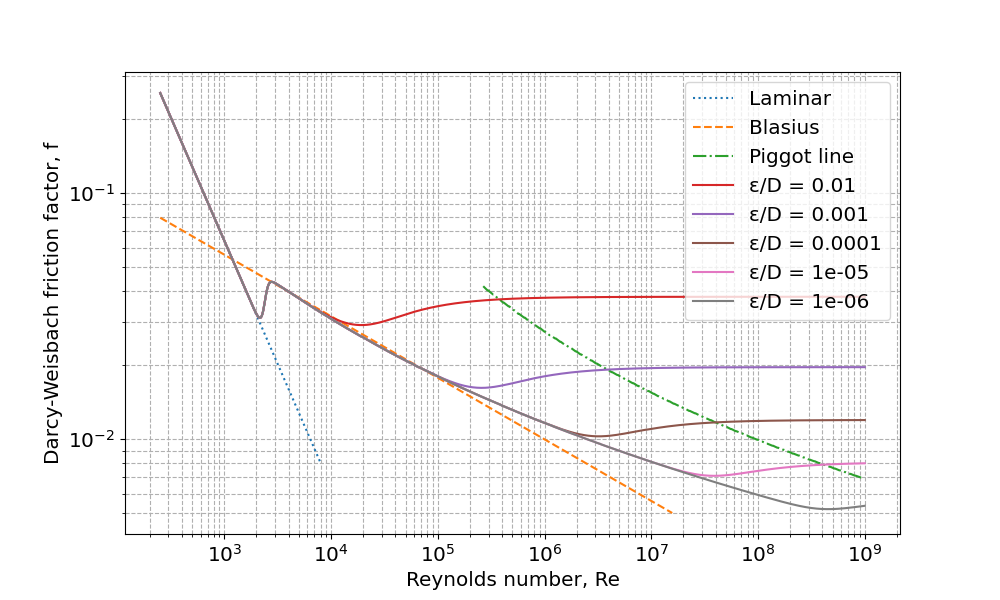
\includegraphics[width=0.49\textwidth]{moody_afzal.png}
\caption{Moody diagram showing the friction factor as a function of the Reynolds number. The Piggot line
marks the transition between inflectional- and fully-turbulent behaviour\citep{Moody1944}. We use a modified Afzal equation\citep{Cerbus2018}  for the lines of different roughness as this is algebraically the most convenient of several which match the inflectional nikuradse behaviour\citep{Allen2007,Goldenfeld2006}}
\label{fig:moody}
\end{figure}

\begin{enumerate}
    \item At the left-hand side of the Moody diagram is the laminar regime, which follows the analytical result of the Hagen-Poiseuille equation regardless of the roughness of the pipe (dotted line). 
    \item In the middle, between the laminar line (dotted) and the Piggot line (dash-dotted) there is the partially-turbulent regime. Most real gas distribution pipes operate in this regime.
    \item At the right-hand side is the fully-turbulent regime, in which the friction factor depends only on roughness, and is independent of $Re$ (horizontal lines to the right of the Piggot line).
\end{enumerate}

Figure~\ref{fig:moody} shows lines for pipes of different 
roughnesses\footnote{There are at least 50 different semi-empirical equations which approximate the implicit Colebrook equation but these are simply mathematical fits and ignore the fact that  the Colebrook equation itself does not describe experimental data to better than $\pm$~15\%~\cite{Allen2007, Cerbus2018, She2012}.  
} 
 for relative roughness values of 10$^{-2}$, 10$^{-3}$, 10$^{-4}$, and 10$^{-5}$. 
%Smooth pipes are defined as those where $\epsilon/D < 10^{-5}$, for which the gas flow is partially-turbulent for $Re < 10^5$.

The minimum visible  at Re $\approx$ 2,300  is where the flow transitions from laminar to turbulent\citep{Allen2007}. 

%The difference in values of $f$ across this gap may be as low as 0.02, in specifically prepared test specimens, or as high as 0.06.

%The full dependence of the friction factor on $Re$ and the relative roughness of the pipe for all fluids in pipes may be determined from the underlying physics by the Goldenfeld function~\cite{Goldenfeld2006}.

\subsection{Regimes in the distribution network }
\label{sec:service}

Distribution networks for natural gas\footnote{Numerical evidence is from the Netherlands\citep{Schouten2004} as UK gas network data is now redacted by the regulator.
} are designed to run in the turbulent regime at peak design flow, with gas velocities in the range 8-12 m/s. 
A general guideline for all gas networks is that the gas velocity should be between 5 and 10 m/s and always less than ~20 m/s to prevent erosive wear by dust particles\citep{Schouten2004,Tabkhi2008,Ejo2020, Abbas2021}.

The pressure drop, about 40~mbar, in the domestic connection is low compared with the absolute pressure, about 1 bar; so the behaviour does not change significantly along the pipe.

The maximum Reynolds number expected within the transmission may be calculated from the natural gas properties, the maximum velocity of 20~m/s, and the maximum pipe diameter of 630~mm\citep{GPS2008}.
This is a value of $Re = 1.0\times10^6$, which is in the middle of the partially-turbulent regime, as per Figure~\ref{fig:moody}.

At the other end of the scale is the domestic connection,
%to the distribution network, 
which in the UK is typically a 35~mm tube of drawn copper, steel, or polyethylene\citep{dodds2013}.
A typical domestic boiler in the UK is rated at 30~kW\citep{GASTEC2009, Bennett2020}.
The energy supply equation~\eqref{eqn:energysupply}, as well as the material properties used in Section~\ref{sec:velocity}, allows us to calculate that the gas velocity of natural gas in this situation is $v$=0.838~m/s, and the Reynolds number is $Re$=2363.
This places the flow at the lower end of the partially-turbulent regime.

Replacing natural gas with hydrogen in any piping system will always reduce the Reynolds number, because while the velocity increases, the density decreases significantly more, and the dynamic viscosity of also decreases\footnote{We use a simple molar fraction weighted approximation for the viscosity of gas mixtures, as that is adequate for the purpose of this paper. For modelling higher pressure transmission networks, a much more complex Chapman-Enskog or corresponding states\citep{coolprop} model would be required.}.
See Section~\ref{sec:nonblasius} for these calculations.

Calculating the Reynolds number for the domestic connection with pure hydrogen gives a value of at 970, quite definitely in the laminar flow regime where the pressure drop is linear in velocity.
Therefore we need to consider multiple regimes that are applicable to different sections of the distribution network.

\subsection{Partially-turbulent flow}

The partially-turbulent regime in Figure~\ref{fig:moody} is between the laminar flow line and the 
Piggot line\footnote{Piggot observed this relationship between $Re$ and relative roughness ($\epsilon/D$) which is the point at which fully turbulent flow develops.}.
It was first reported in the discussion published at the end of the original Moody paper\citep{Moody1944}. 
Behaviour in the partially-turbulent regime in Figure~\ref{fig:moody} may be further subdivided:
\begin{itemize}
    \item The transition from laminar to turbulent flow, where the friction factor curve has a minimum\footnote{This dependence is a characteristic of the physics of critical systems as shown by Goldenfeld\citep{Goldenfeld2006}.}.
    \item The Blasius sub-regime, shown as a dashed straight line.
    \item The departure from the Blasius line, but where the friction factor continues to vary with Re, before the Piggot line is reached.
\end{itemize}

For $Re$ less than $2\times10^5$ the friction factor follows the Blasius law, for more than $2\times10^5$ it diverges~\cite{Allen2007} but still depends on $Re$ until the Piggot line.
The friction factor $f$ in the Blasius sub-regime is given by equation~\eqref{eqn:darcywiesbach}\citep{Bennet2017}.

\begin{equation}
\label{eqn:blasius}
f_{Blas} = 0.079 \times Re^{-1/4}
\end{equation}

For smooth pipes, such as steel or polyethylene with a relative roughness of $10^{-5}$, the friction factor $f$ for gas in distribution pipes varies between 0.008 and 0.045, as can be seen from Figure~\ref{fig:moody}.

\subsection{Pressure drop in the Blasius sub-regime}
\label{sec:pressuredrop}

In the range of $Re \in (2\times10^3,2\times10^5)$, we can combine the Darcy-Weisbach equation~\eqref{eqn:darcywiesbach}, the Blasius equation~\eqref{eqn:blasius}, and the Reynolds number definition~\eqref{eqn:re}, to give the dependence of pressure drop on all relevant parameters:

\begin{equation}
\label{eqn:pdrop0}
\Delta P = \left ( \frac{4 \cdot 0.079}{D^{5/4}}\right ) \cdot \rho^{3/4} \cdot \mu^{1/4} \cdot v^{7/4}
\end{equation}

In equation~\eqref{eqn:pdrop0} the terms in brackets are constant when comparing any fluids in the same pipe. 
The remaining terms show the dependency on 
%material 
the
properties, given in table~\ref{tab:dyn}, and the gas velocity.
The  material parameter $\rho^{3/4} \times \mu^{1/4}$ is almost independent of 
temperature\footnote{
Varying by less than $\pm$~1.2\% over the range -40$^\circ$C to +50$^\circ$C, see \ref{sec:blasiusparam}.
}.

Using equation~\eqref{eqn:pdrop0} for the two fuels gives equation~\eqref{eqn:pdropratio}.

\begin{table}
\centering
\begin{tabular}{r|c|l}
& Density & Dynamic viscosity \\
& [kg/m$^3$] & [$\mu$Pa$\cdot$s] \\
\hline
H$_2$ & 0.0914 & 8.509 \\
NG & 0.0836 & 10.374 \\
\hline
ratio & 0.1902 & 0.8202
\end{tabular}
\caption{\label{tab:dyn}Densities and dynamic viscosities at 8$^\circ$C and 40~mbar }
\end{table}

\begin{equation}
\label{eqn:pdropratio}
    \left(\frac{\Delta P_{H_2}}{\Delta P_{NG}}\right)_{Blasius} = 
    \left(\frac{\rho_{H_2}}{\rho_{NG}}\right)^{3/4} 
    \left(\frac{\mu_{H_2}}{\mu_{NG}}\right)^{1/4} 
    \left(\frac{v_{H_2}}{v_{NG}}\right)^{7/4}
\end{equation}

Unlike equation~\eqref{eqn:velocityratio} for the velocity ratio, equation~\eqref{eqn:pdropratio} directly includes the density, $\rho$, as it is an important factor in the inertial forces giving rise to pressure drop.
Using the material properties from table~\ref{tab:dyn} and the velocity ratio from Section \ref{sec:velocity} for hydrogen and natural gas, we find the ratio of pressure drops of the two gases to be:

\begin{equation}
\label{eqn:pdropratiovalue}
    \left(\frac{\Delta P_{H_2}}{\Delta P_{NG}}\right) = 
    0.1902^{3/4} \times 0.8202^{1/4} \times 3.076^{7/4} = \mathbf{1.294}
\end{equation}

Now we can perform the iterative calculations to work out the average pipe pressure that was used in Section~\ref{sec:avpressure}. 
The distribution network is controlled such that the low pressure end, $P_{min}$, is maintained at 20~mbar\citep{dodds2013}, and we have been using an average pressure for natural gas of $P_{av,NG}=40$~mbar\citep{utonomy23}.
The average pipeline pressure is related to the minimum pressure and the pressure drop by:

\begin{equation}
    \label{eqn:avpressure}
    P_{av} = \tfrac{1}{2}(P_{min}+P_{max}) = P_{min} + \tfrac{1}{2} \Delta P
\end{equation}

This may be combined for both hydrogen and natural gas to calculate the average pressure for hydrogen:

\begin{equation}
    \label{eqn:avpressurecalc}
    P_{av,H_2} = P_{min} + ( P_{av,NG} - P_{min} ) \left(\frac{\Delta P_{H_2}}{\Delta P_{NG}}\right)
\end{equation}

Thus the iterative process is:
\begin{enumerate}
    \item Make an initial guess for the value of $P_{av,H_2}$
    \item Use this pressure in equation \eqref{eqn:velocityratio}.
    \item Use this velocity ratio in equation \eqref{eqn:pdropratio}.
    \item Use this pressure drop ratio in equation \eqref{eqn:avpressurecalc}.
    \item repeat steps 2 to 4 until the value of $P_{av,H_2}$ converges.
\end{enumerate}

The converged value is $P_{av,H_2}=45.88$~mbar, which is the value that was used in Section~\ref{sec:avpressure} to be representative of a typical high-flow situation. 
This gives a maximum pressure within the pipe of 71.75~mbar, which is close to but below the maximum rating of 75~mbar\citep{dodds2013}.

\subsection{Laminar regime}
\label{sec:laminarturbulent}

Below a Reynolds number of $2\times10^3$, all pipes regardless of roughness should exhibit laminar behaviour. 
The friction factor in this regime can be derived analytically from Poiseuille flow as:

\begin{equation}
\label{eqn:flaminar}
    f_{Lam} = \frac{64}{Re}
\end{equation}

This may be used in place of equation~\eqref{eqn:blasius} for  expressions for the pressure drop ratio and the compressor power ratio in the laminar regime with different exponents on the 3 terms:

\begin{equation}
\label{eqn:pdropratiolam}
    \left(\frac{\Delta P_{H_2}}{\Delta P_{NG}}\right)_{Lam} = 
    \left(\frac{\rho_{H_2}}{\rho_{NG}}\right)^{0} 
    \left(\frac{\mu_{H_2}}{\mu_{NG}}\right)^{1} 
    \left(\frac{v_{H_2}}{v_{NG}}\right)^{1} = \mathbf{2.537}
\end{equation}

This value was calculated using the iterative method of section~\ref{sec:pressuredrop}, in the limit that flow is slow enough that  $\Delta P \ll P_{min}$, as we have no reasonable estimate of average pressure in a laminar slow situation. 
The corresponding velocity ratio in the laminar regime is 3.094.

\subsection{Fully turbulent regime}
\label{sec:departure}

At sufficiently high Reynolds number, flow enters the fully turbulent regime where $f$ is independent of $Re$.
For smooth drawn tubing with ($\epsilon/D$) = $5\cdot10^{-5}$ this transition is at $Re = 3.5\cdot10^8$, determined by the Piggot relationship in equation~\eqref{eqn:piggot}. 

\begin{equation}
\label{eqn:piggot}
   \frac{3500}{\epsilon/D} = Re
\end{equation}

As the maximum obtainable Reynolds number in the distribution network is $10^6$ from section~\ref{sec:service}, there is no way to achieve the fully turbulent regime without exceeding at least one of the network's design limitations.

\subsection{General relationships}
\label{sec:nonblasius}

While the values derived above work well for cases in which the fluid regime is well defined, there are gaps between these regimes. 
The transition from laminar to partially turbulent behaviour is notoriously complex, however recent works have made an effort to understand this transition on a fundamental level\citep{Goldenfeld2006, She2012}.
There is also a wide section of the partially-turbulent regime from $Re = 2\times10^5$ to $3.5\times10^8$ where the friction factor is not yet constant but also does not follow the Blasius equation.
We hypothesise that much of the UK gas grid should be in this non-Blasius sub-regime.

%Furthermore, 
Replacing natural gas with hydrogen can change the flow regime entirely.
In the service pipe modelled in section~\ref{sec:service}, the regime was partially turbulent with natural gas, yet switching to hydrogen resulted in laminar flow.

For the  gas velocity change of approximately 3$\times$ from natural gas to hydrogen, depending on regime, there is a Reynolds' number shift which depends on the relative velocity changes and also on the relative densities of hydrogen and natural gas:

\begin{equation}
\label{eqn:reshift}
    \left(\frac{Re_{H_2}}{Re_{NG}}\right) = 
    \frac{
        \left(\frac{\rho_{H_2}}{\rho_{NG}}\right)
        \left(\frac{v_{H_2}}{v_{NG}}\right)
    }{
        \left(\frac{\mu_{H_2}}{\mu_{NG}}\right)
    }
\end{equation}


Using the modified Afzal equation for the friction factor, the increase in pressure drop may be plotted against the any pipeline Reynolds number for natural gas in Figure~\ref{fig:pressuredrop}.
The Reynolds number for hydrogen will be less than the x-axis value by equation~\eqref{eqn:reshift}, for the same pipe geometry, and this has been incorporated into the calculations. 

\begin{figure}[htb]
\centering
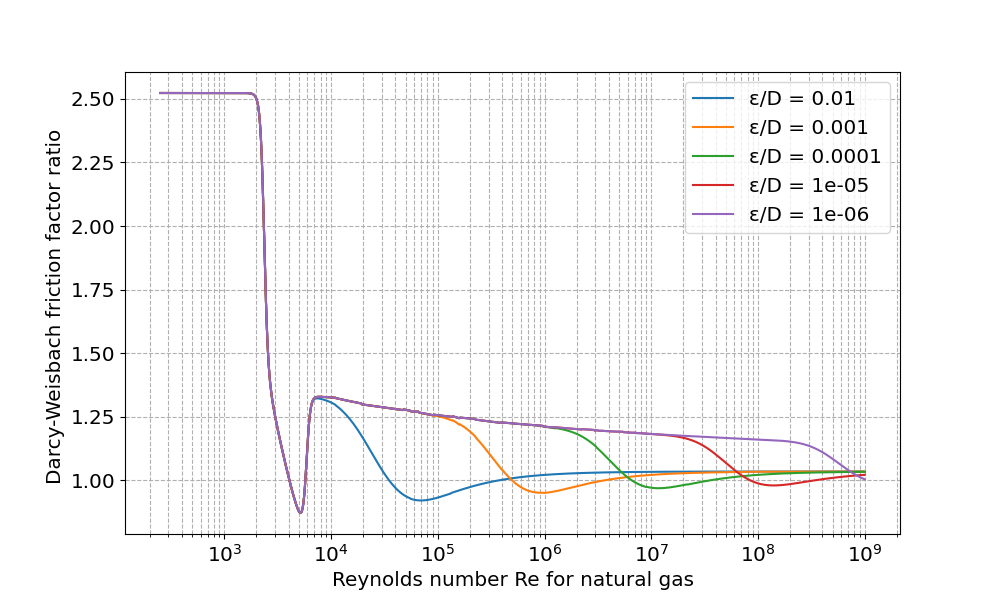
\includegraphics[width=0.49\textwidth]{p2_h2_ratio.png}
\caption{The increase in pressure drop as a function of the Reynolds number for natural gas, when replacing natural gas with hydrogen. The curves for the friction factor and compressor power follow the same trend, but are scaled by combinations of the ratios of density, viscosity, and velocity, which are independent of the Reynolds number. These curves make use of the assumption of incompressible flow, so should be treated with caution for gasses at very high Reynolds numbers.}
\label{fig:pressuredrop}
\end{figure}

Figure~\ref{fig:pressuredrop} shows that at locations and times where the natural gas flow is slower, there will be a proportionally larger increase in the pressure drop by switching to hydrogen.
The dip at $Re\approx5\times10^3$ is where the switch to hydrogen causes the flow to change from turbulent to laminar, which can result in a decrease in the pressure drop in the pipe.
The transition is effectively a time-average of an unstable switching between these two states, but it is not practical to design systems to make use of this.

%This is similar to the existing situation with natural gas, where during off-peak demand hours the gas velocity drops and the Reynolds number drops. 

The increase in the compression power for hydrogen over natural gas has been noted by Schouten\citep{Schouten2004} and others, but only for fully-turbulent conditions. 
The increase in friction factor and the consequent increase in compressor power required has not previously been recognised.

\subsection{Pumping power}
\label{sec:comppower}

The pressure drop of a flowing fluid arises from frictional losses. 
The pumping power, $W$, required to overcome these losses for an incompressible fluid is the product of the pressure drop and the volumetric flow rate. 
In a pipe\citep{Bennet2017} this is:

\begin{equation}
\label{eqn:power}
 W = \Delta P \cdot v \cdot A 
\end{equation}

The proportional increase in the compression power requirement when switching from natural gas to hydrogen is therefore the ratio of this equation for the two gasses:

\begin{equation}
\label{eqn:powerratio}
    \left(\frac{W_{H_2}}{W_{NG}}\right) =
    \left(\frac{\Delta P_{H_2}}{\Delta P_{NG}}\right)
    \left(\frac{v_{H_2}}{v_{NG}}\right)
\end{equation}

As we have shown, the velocity ratio is largely independent of the flow regime and depends mostly on the thermodynamics of combustion, this means that the ratio of compressor power follows the exact same trend as the ratio of pressure drop does in Figure~\ref{fig:pressuredrop}, with the values all scaled up by the velocity ratio, 3.076.

We can calculate individual values for the three major regimes.
In the Laminar regime $(W_{H_2}/W_{NG})_{Lam} = 7.76$, in the Blasius regime $(W_{H_2}/W_{NG})_{Blas} = 3.98$, and in the fully turbulent regime $(W_{H_2}/W_{NG})_{FT} = 3.19$.
Even in the dip where the pressure ratio is less than one, the compressor power still increases by approximately 2.5$\times$ due to the much faster gas velocity for hydrogen.

Since we expect most of the flow in the distribution network to be in the Blasius regime, this tells us that the energy required to deliver hydrogen through the distribution network will be 3.98$\times$ greater than for natural gas.

\section{UK distribution capabilities}
\label{sec:distcapable}

%Although the standard maximum pressure for the Low Pressure (LP) distribution grid is 75~mbar
Much of the older network runs at only 50~mbar~\cite{ARUP2023} to reduce leakage, where this still gives adequate pressure (20~mbar) at the most distant user. 
This could be increased up towards the maximum 75~mbar level with new polyethylene pipe which is less prone to leaks\citep{ARUP2023}. 

The UK domestic gas demand\citep{DESNZ2023a} peaked in 2004 at 34,035 toe\footnote{toe = tonne of oil equivalent, 1 toe is equal to 11.63~MWh} and in the most recent cold winter year (2021) it was 26,275 toe. 
This means that the network today can cope with an annual demand of natural gas at least 29.5\% higher than it currently supplies.
While it is possible that during the peak hourly demands of 2004 and 2021 this ratio was less than the annual ratio, we can only expect that this over-capacity will continue to grow into the future as more houses get insulated, upgraded or replaced and also due to climate change reducing the heating demand overall\citep{Christidis2021}. 

\section{Conclusions}
\label{sec:conc}

While it is clear that burning hydrogen for heat in a boiler, or even in a combined heat and power cell, is almost a use of last resort\citep{Rosenow2024,Liebreich2021}, there appear to be no pressure difficulties with delivering pure hydrogen using the existing UK distribution network. This paper shows that the velocity is similar to that which had previously been thought but that the pressure drop and power requirement are higher.

It has not previously been noted that:
\begin{itemize}

    \item Burning hydrogen means that care must be taken to reduce the condensation temperature of the condensing boiler as much as possible because a greater proportion of the combustion energy is in the form of condensible water.
    \item Using hydrogen reduces the Reynolds' number of the flow rather than increasing it.  
    \item There is a slight effect of increasing the mean pressure, and thus the energy density, of the hydrogen because it requires a 29\% higher pressure gradient to be delivered.
    \item The Blasius material parameter $\rho^{3/4} \cdot \mu^{1/4}$ has a very low temperature dependence, meaning that our conclusions on relative pressure drop and the relative compression power are largely insensitive to temperature whilst the Blasius equation holds.
    \item As well as the low pressure system investigated here in detail, we hypothesise that the Medium and Intermediate Pressure distribution pipes are operating for much of the time in the partially-turbulent regime.
\end{itemize}

\section{References}
\bibliography{h2pipe}


\section*{Acknowledgements}
\label{sec:ending}

We thank Ian Ellerington for posing the question in 2013 of recalculating the velocity ratio, and John Baldwin of CNGservices for providing the natural gas composition.

\appendix

\section{Software used in this study}
\label{sec:oursoftware}
%This document is written in \LaTeX{} using the 
%collaborative  editor  \url{https://www.overleaf.com}.  
The python code and input data is published on GitHub: \url{https://github.com/PhilipSargent/h2-in-pipes} under the MIT open source license\citep{Sargents_github}.

\section{Compressibility}
\label{appendix:gasprops}
All calculations in this paper have used an equation of state and  mixing rules appropriate to the pressure and temperature for each pure gas or blend studied. Individual corrections are small, but they multiply together to make a significant difference.

To calculate the compression factor as a function of temperature and pressure, and for gases such as natural gas composed of several different compounds, one needs an equation of state.
The low pressures and ambient temperatures of the distribution grid mean that several different equations of state are all sufficiently accurate.

Lozana $et$ $al.$ have recently reviewed\citep{Lozana2022}  the relevant equations of state and there are a bewildering variety of suitable functions.

\label{sec:eqnofstate}
 In this paper we use the 1978 Peng-Robinson equation of state\citep{Tabkhi2008, Abbas2021}, with temperature dependent binary interaction parameters and no volume translation corrections.
 For the exact calculation method used in this paper, see 
%  \ref{sec:gasmix} and
 the code\citep{Sargents_github}. 



\section{Upgrading UK Boilers}
\label{appendix:more-boilers}
\label{appendix:h2upgrade}
%\subsection{Hydrogen upgrade condensing boilers}

In the most recent English housing survey\citep{ehs21}, approximately one tenth (7/(59+7)) of domestic boilers on piped-gas were non-condensing and nine-tenths condensing: 
``the proportion of dwellings with a standard boiler decreased from 9\% in 2020 to 7\% in 2021, while the proportion with a condensing-combination boiler has increased from 57\% to 59\% in the same period".

However there are no statistics on how many of the condensing boilers have correctly-adjusted $50^\circ$C return-flow settings with appropriate weather compensation. Anecdotally, the proportion is very small, very likely less than 5\%. So a reasonable estimate would be that the return temperature is set to $50^\circ$C for 5\% of the condensing boilers and to $70^\circ$C for 95\% of the them. There is no condensing for the non-condensing boilers so their efficiency is simply that at  a `condensation' temperature of $100^\circ$C.

We will assume
\begin{itemize}

    \item That 4\% of boilers are already perfectly adjusted, and the only change will be the multiplier of 0.974$\times$ from the change in fuel condensation behaviour
    \item That 86\% of boilers will go from a condensing temperature of $70^\circ$C (87.44\% with NG) to $50^\circ$C (93.69\% with hydrogen), a multiplier of  0.933$\times$
    
    \item That 10\% of boilers will change from an efficiency of  86.20\% (non condensing) to a fully-condensing, properly adjusted reflow temperature of 50$^\circ$C (93.69\% with hydrogen), a multiplier of 0.920$\times$
\end{itemize}
The population weighted efficiency multiplier is thus 0.933$\times$.

\subsection{Published boiler efficiencies}
Boiler efficiency\citep{Bennet2017} is  measured either in a test rig at steady-state load, or estimated as a seasonal average as-installed in a house with a typical daily heating cycle and weather pattern. Repeated on- and off-periods increase losses\citep{saty2018}. Boiler manufacturer published efficiency values may be legally-required in some jurisdictions to be a seasonally-adjusted average number.


\section{Viscosities and temperature}
\label{sec:viscosities}
The viscosities of pure components are calculated from experimental data as a least-squares fit to a power law dependence on absolute temperature. Ideal gases have a power law relationship where the exponent is 0.5, the real gases here have exponents between 0.66 and 1.08. The viscosity of the gas mixture is a molecular fraction weighted average\citep{Krieger1951} of the viscosities of the components.

\begin{figure}[htb]
\centering
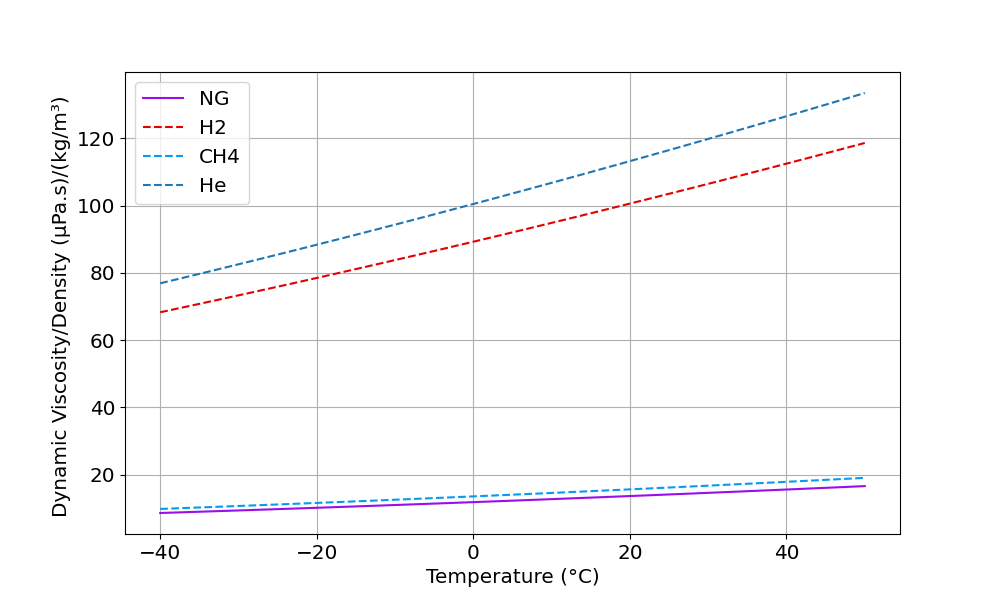
\includegraphics[width=0.49\textwidth]{peng_re.png}
\caption{Plot of kinematic viscosity: the ratio of dynamic viscosity and density, as a function of temperature at 1.06825 bar}
\label{fig:peng_re}
\end{figure}

Figure~\ref{fig:peng_re} shows the temperature dependence of the kinematic viscosities (the ratio of density to dynamic viscosity) of  the natural gas blend, hydrogen and methane. This shows why it is important to do these calculations at a well-chosen reference temperature rather than using textbook values which may have been measured at a variety of different temperatures.

In the UK the ground temperature of the buried LP network is likely to stay in the range 5 to 15$^\circ$C all year\citep{MacKay2008}.



\subsection{The Blasius materials property}
\label{sec:blasiusparam}
Note that the term $\rho^{3/4} \cdot \mu^{1/4}$ in equation \eqref{eqn:pdrop0} is a materials' property which depends on temperature and pressure. We define this property as B, the Darcy-Weisbach Reynolds-Blasius parameter in equation \eqref{eqn:defnb}; or abbreviated to the 'Blasius parameter'.

\begin{figure}[htb]
\centering
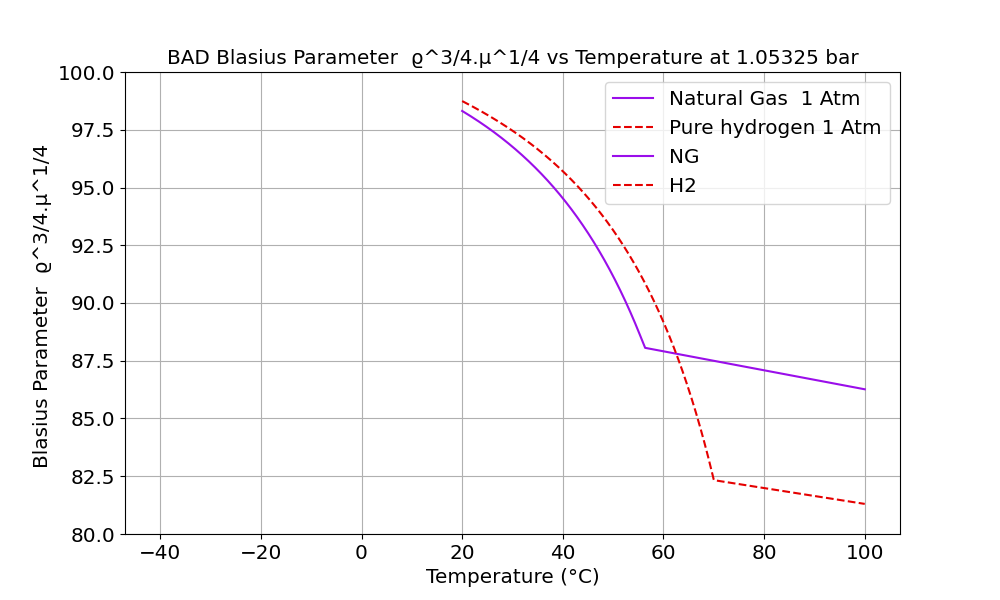
\includegraphics[width=0.49\textwidth]{peng_bf.png}
\caption{Blasius Parameter  $\rho^{3/4} \cdot \mu^{1/4}$ ((kg/m)$\cdot$(m$\cdot$s)$^{-4}$ )}
\label{fig:blasiusparam0}
\end{figure}

\begin{equation}
\label{eqn:defnb}
B =  \rho^{3/4} \cdot \mu^{1/4} 
\end{equation}
where $\rho$ is the density and $\mu$ is the dynamic viscosity.

Somewhat surprisingly, this materials' property has only a slight dependence on  temperature as the dependencies of density and viscosity act in opposite directions. 


Also surprisingly, all the gases in the study have very similar dependence such that the normalised Blasius parameter, where the value for each gas is divided by the value for natural gas, is very nearly independent of temperature, varying less than 1.2\% between -40$^\circ$C and +50$^\circ$C.
%see Figure~\ref{fig:blasiusparam}.

%\begin{figure}[ht]
%\centering
%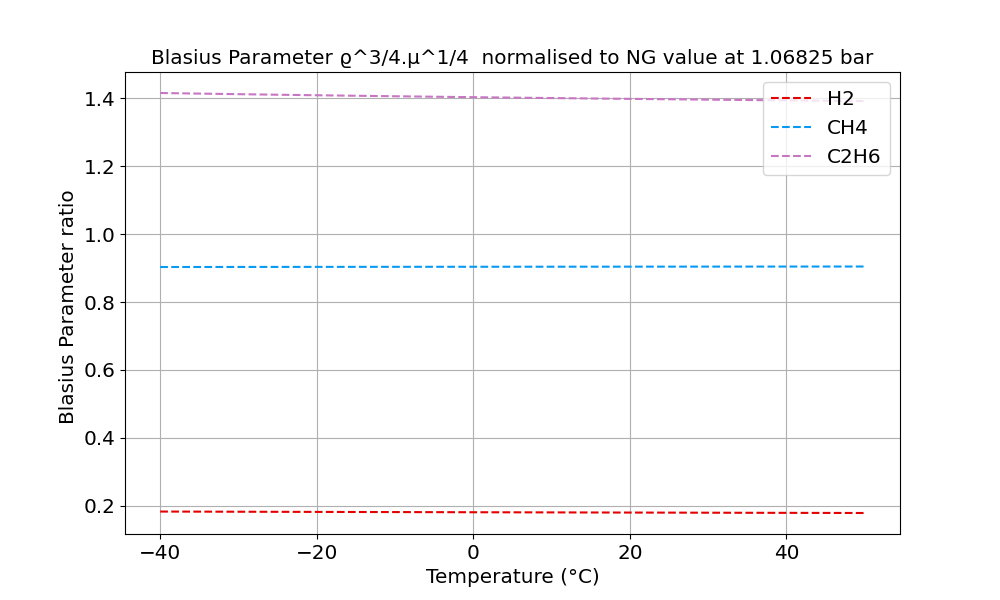
\includegraphics[width=0.49\textwidth]{peng_bf_NG.png}
%\caption{Ratio of  Blasius Parameter  to that of natural gas NG }
%\label{fig:blasiusparam}
%\end{figure}

This means that results calculated using the Blasius parameter, the relative pressure drop  and the relative compression power requirement, are independent of temperature in the distribution grid.

\section{Dew point and partial pressure}
\label{sec:partial pressure}
Our calculations produce the partial pressure of water vapour in the flue gas, but we need the dew point. The two are related by standard tables of the  saturation vapour pressure of water\citep{Perry2008}: the pressure at which water vapour is in thermodynamic equilibrium with its condensed state.

The range of atmospheric pressure in the UK means that the dew point of the flue gas varies   $\pm1.4^\circ$C, which affects the maximum efficiency.

~\\
\fbox{\begin{minipage}{20em}
The published paper is likely to be limited to 12 pages. The bibliography should compress slightly as the URLs get rendered more compactly in the final format.
\end{minipage}}
\newpage % disposable content beyond this point

\section{The Peng-Robinson calculations}

Equations of state for gas mixtures are still an active research area\citep{Lozana2022} and there is continual development of alpha functions, interaction parameters and mixing rules e.g. Pina-Martinez $et$ $al.$\citep{Pina-Martinez2019}.

\subsection{Calculating the properties of a gas mixture}
\label{sec:gasmix}
The higher heat capacity and the mean molecular weight of the Fordoun natural gas are calculated from a mole fraction weighted sum of those properties of the component pure gases.

The compressibility and density of the natural gas are calculated for a given temperature and pressure using the Peng-Robinson equation of state: 

\begin{enumerate}
\item The Peng-Robinson\citep{Pina-Martinez2019} parameters $a$ (attraction) and $b$ (repulsion) for each pure component  at a given temperature are calculated from the critical temperature $T_c$, the critical pressure $P_c$, and the $omega$ coefficient (a measure of the molecule asphericity) of each pure gas.
    \item the coefficient $b$ of the mix is   the weighted sum of the $b$ values of the component gases, where the weights are the mole fractions. 
    \item The temperature dependent binary interaction parameter k is calculated using the Courtinho method~\cite{Privat2023} from the $b$ value of each gas in a pair. For an 11 component gas there are 55 pairwise interactions.
    \item The $a$ values are calculated as the weighted sums of the geometric means of the pair-wise values of $a$ between each pair of components. The weights are the mole factions of each pair multiplied together, times the value (1-$k$)
    \item The effective $T_c$, $P_c$ and $omega$ of the natural gas, the pseudo-component,  are calculated from the $a$ and $b$ values for the mix for the given temperature
    \item the compressibility and thus the density of the natural gas is calculated using the effective $T_c$, $P_c$ and $omega$ values.
\end{enumerate}
The precise algorithm is in the code on GitHub~\cite{Sargents_github}.




\section{Wobbe number and reference temperatures}
\label{sec:wobbe}
At 15$^\circ$C the Fordoun gas has  a density of 0.81507~kg/m$^3$, an \textsc{hhv} of 39.8902~MJ/m$^3$, and a Wobbe number
\footnote{The Fordoun gas is thus
centrally within the regulatory limits.
} of 49.97451~MJ/m$^3$.

In the UK 15$^\circ$C is the temperature for assessing allowable\footnote{'The multiplicity of ``standard reference conditions" of temperature, pressure and humidity (state of saturation) used in the measurement of natural-gas quality and quantity can cause much confusion', ISO 13443\citep{ISO13443}} Wobbe limits\citep{GS(M)2023,Lander2017}. Wobbe values of fuel gases are sensitive to temperature via the effect of temperature on gas density and molar volume and the distinction between 15$^\circ$C and the industry informal standard of 0$^\circ$C is significant. However, despite ISO 13443, the 25$^\circ$C reference heat  of combustion always seems to be used in practice for Wobbe calculations.
\footnote{ ISO~13443  defines standard reference conditions of 15$^\circ$C and 1.01325~bar for use with natural gases and natural gas substitutes. ISO 6976 was substantially revised in 2016 and data, especially Wobbe data, from papers published before then should not be re-used without being re-evaluated\citep{Lander2017}
} . 

This paper does not use Wobbe numbers in any of the calculations. 


\section{Laminar flow}
\label{appendix:laminar}

If the gas velocity at night is sufficiently slow that both the natural gas and the hydrogen fall within the laminar flow regime, then the pressure drop is linear in both velocity and viscosity. The viscosity ratio is 0.8209 at 8$^\circ$C and the velocity ratio, which is unchanged, is 3.076. Thus, the pressure drop ratio is 2.523 .

The compressor power required to deliver it will be the velocity ratio times the pressure drop ratio, i.e. 7.763$\times$ greater.

\begin{table}[htb]
\centering
\begin{tabular}{l|r}
 & Ratios for H2/NG \\\hline
velocity & 3.076 $\times$  \\
pressure drop & 2.523 $\times$  \\
power reqd. & 7.763 $\times$  \\
\hline
\end{tabular}
\caption{\label{tab:laminar}Laminar flow -- at 8 C}
\end{table}


\section{Lower Heating Value (LHV) and process heat}
\label{sec:processheat}
Some users on the distribution network use gas for process heat;  for an oven, furnace or kiln. Replacing natural gas with hydrogen for these users means that the velocity factor, the ratio of the gas velocity for hydrogen and natural gas, is the ratio of the gases' LHV  in kJ/$m^3$.

There is no generally agreed  way of defining LHV unless the exit temperature of the flue gas is specified. If the latent heat of the water is simply subtracted from the \textsc{hhv}, that is equivalent to saying that the flue gas exits at 25$^\circ$C which would be quite wrong. For a bread oven it would be about 190$^\circ$C whereas a pottery kiln could be up to 1,400$^\circ$C (though in that case the flue gases should, one would hope, go into a heat recovery system and also be used to dry wet clay).

\section{Mean pressure corrections}
\label{sec:mean-pressure}
In the main paper we have shown that the pressure drop of the hydrogen in the distribution pipe is affected by the required velocity of the hydrogen, but also that the velocity is slightly modified by the mean pressure, which depends on the pressure drop. Because this dependence is slight we have been able to iterate to find an exact solution - always with the assumption that the whole pipe is experiencing the same flow regime.

However we have implicitly assumed that the pressure gradient along the pipe is linear by assuming that the mean pressure is half-way along the pipe and that that is representative of the average behaviour of the gas. This is not true, even for ideal gases.

For the service pipe with pressures below 75~mbar this correction is slight, but for intermediate pressure distribution pipes at 7~bar the correction should be calculated more accurately.

At steady state there is the same amount of gas entering the pipe as leaving, so if the pressure (and thus density) is higher at the inlet (as it must be), the velocity must be greater at the exit where the pressure (and density $\rho$) is lower. For an ideal gas the product $\rho$v is a constant: as the pressure drops and the density drops (linearly), the velocity must increase.  The Reynolds' number is proportional to $\rho$v, which is a constant along the pipe so, for an ideal gas,  the friction factor is also constant along the pipe.

The local pressure drop ($\delta$P/$\delta$x in Pa per mm) at a point increases along the pipe, so the velocity increase (in m/s per mm) also increases. The gas accelerates as it flows through the pipe.

But according to the Darcy-Weisbach relation (equation \ref{eqn:darcywiesbach}) the pressure gradient at any point is proportional to  $\rho$v$\cdot$v, so as the velocity increases, the local pressure drop at each point increases. This means that the local pressure along the pipe is a monotonic, convex curve: it is flatter at the higher pressure inlet end. The point at which the pressure drops to the mid-point of the pressures at each end is not the middle of the pipe, but some way towards the exit end, perhaps 2/3 of the way along. This can be solved analytically, but to be accurate we need to take into account the compressibility of the gas which itself depends on the absolute pressure. So more than half the gas in the pipe is experiencing a higher pressure than the assumption made in the paper for the service pipe, so the gas is on average a little denser. but this does not mean that the velocity is lower: that only matters at the point of delivery, at the pipe exit.

\section{16km visualisation}
\label{sec:18km}
A way of visualising the network characteristics is to imagine a single 110~mm diameter pipe carrying the natural gas with 75~mbar pressure at one end and 20~mbar pressure at the other with a velocity of 1.73~m/s\footnote{
This is the gas velocity when the domestic meter maximum of 6~$m^3$/s of gas is delivered to a single household through a 35~mm pipe.
}  and $Re$ = 11,849. We use the Darcy-Weisbach equation (equation \eqref{eqn:darcywiesbach}) and rearrange to get


\begin{equation}
\label{eqn:18km0}
Length = \left ( \frac{2 \cdot \Delta P}{0.079}\right ) \cdot \rho^{-3/4} \cdot \mu^{-1/4} \cdot v^{-5/4}  \cdot D^{5/4}
\end{equation}

$ \Delta P = (75 - 20)/1000~bar$

$ \rho^{-3/4} = (0.84148)^{-3/4} \rho: (kg/m^3)$

$ \mu^{-1/4} = (10.37391 \cdot 10^{-6})^{-1/4} \mu:  (\mu Pa.s)$

$ v^{-5/4} = (1.7323)^{-5/4} v: (m/s)$

Solving this we find that this pipe would be about 16~km long .

If we imagine that this was representative of the UK gas demand in 2004, then in 2021 the reduced amount of gas (77.2\%) would mean that the velocity would reduce in proportion and the pressure drop would reduce. So if the high pressure end was maintained at 75~mbar the  pressure at the low pressure exit would rise to 40.03~mbar. 

If we now replaced the gas with pure hydrogen  delivering the same useful energy flowing at $3.076\times$ the velocity then the pressure at the domestic end would be 29.7~mbar with a Reynolds' number of 4,868.
So with hydrogen, even though it requires a higher pressure drop, this example network would still have `headroom' of 9.7~mbar above the domestic exit limit of 20~mbar.

\section{UK Boilers in yet more detail}
\label{appendix:yetmore-boilers}

The gradient of the condensation curve of Figure~\ref{fig:efficiency} is shown in Fig. \ref{fig:gradient}. For a hydrogen boiler, the increase in efficiency per degree cooling peaks at 0.009~\%/K at the dew point.


\begin{figure}[htb]
\centering
\includegraphics[width=0.49\textwidth]{peng_dη.png}
\caption{How the efficiency of the boiler changes for each degree that the condensation temperature reduces.}
\label{fig:gradient}
\end{figure}

\subsection{Enriched air}
Burning a fuel in pure oxygen always gives a slight benefit of efficiency because the heat loss in the sensible heat of hot nitrogen is avoided, but this is rarely worth doing for the slight extra efficiency. However in a condensing boiler, removing some of the nitrogen significantly shifts the dew point of the flue gas\footnote{Patent in process} thus a much greater leverage on the efficiency is achieved.

This would have the effect of reducing the  return flow temperature in the heating system without having to modify the radiator circuit. This has a greater effect for hydrogen fuel than for natural gas: shifting the dew point 10$^\circ$C could increase the efficiency from 82.4\% to 89.4\%, a very substantial benefit.

Commercially available domestic oxygen concentrators are now available for medical support, and it would be interesting to see whether a new condensing boiler could be designed to use this technology effectively.


\subsection{Hydrogen upgrade boiler controls}
\label{appendix:h2controls}
When considering a transformation to 100\% hydrogen, every boiler will require replacement or systemic upgrade, and it would be reasonable to expect that as well as setting correct return temperatures, modern weather-compensating controls\footnote{
Weather compensation uses an external thermometer reading to reduce the flow temperature of a boiler on mild days. It can reduce annual fuel requirements by reducing the return flow temperature, the condensation temperature, optimally every day. But it has no effect on the peak demand on the coldest days.
}
would be installed at the same time. This would have a dramatic effect on the energy demand of the UK housing stock and  significantly reduce the quantity of hydrogen required over the  year - though not on cold days during peak demand hours.

\subsection{Dew point and steam tables}
\label{appendix:steam-tables}
There are several explicit formulae which model the vapour pressure of water as a function of temperature, but the dew point temperature is very sensitive to slight inaccuracies. For example, the commonly used Antoine equation would get the dew point incorrect by nearly $2^\circ$C.

In our work we use the Sonntag method\citep{Perry2008}.

\subsection{Solubility of Carbon Dioxide}
\label{sec:CO2solubility}
There is one extra effect which means that the Higher Heating Value for natural gas is a very slight underestimate of what is achievable.

The standard heat of combustion is derived assuming that the resultant gases are in their standard state at $25^\circ$C and one atmosphere. For $CO_2$ this will not be true: in a condensing boiler some of the $CO_2$ will preferentially dissolve in the condensing water and this is (overall) an exothermic reaction generating more heat.

The solubility of $CO_2$ is about 0.004\% mole fraction\citep{Carroll1991} at $20^\circ$C and at a partial-pressure of 0.09~bar (8.94\% mol/mol in Table~\ref{tab:NTSgcombustion}), and it is less soluble at higher temperatures, so the effect on the \textsc{hhv} is very small.

In a boiler burning pure hydrogen, there is no effect as there is no $CO_2$.

\subsection{Boiler overcapacity}
\label{appendix:boilerovercap}
There is likely to be significant heating capacity headroom with existing domestic boilers, which are almost invariably oversized\citep{Bennett2020}
\footnote{Where domestic heating is inadequate, this is almost invariably due to inappropriate ventilation, piping, radiators or controls.}
as shown in Fig \ref{fig-oversize}. 

\begin{figure}[ht]
\centering
\includegraphics[width=0.49\textwidth]{boiler-sizes.png}
\caption{Example data from the Energy Saving Trust\citep{GASTEC2009} illustrating that nearly all UK boilers are oversized.}
\label{fig-oversize}
\end{figure}
However this tells us little about whether the Service Line low pressure distribution network is oversized.

\section{20\% Hydrogen in Natural Gas}
\label{sec:H20-percent}

 UK standards state that boilers installed since 1996 must be capable\citep{H2Blends21} of combusting up to 23\% hydrogen. However when burning 100\% hydrogen, the internals of the boiler would need to be significantly changed because of flame velocity issues.

When considering hydrogen being introduced as a partial blend into the gas network, it is appropriate to assume that the population of boilers will require no systemic maintenance or upgrades if the percentage of hydrogen is 20\% or less as this is the purpose of limiting the addition to 20\%.

All efficiency calculations of properly adjusted condensing boilers assume that the heat exchanger is perfect, with all water condensed at the reflow temperature. In reality there will be an additional loss. When adding hydrogen, the velocity of the $flue$ gas increases by an amount which is quite different from the increase in velocity of the $fuel$ gas. This increased flue gas velocity is likely to degrade the efficiency of the the  exchanger through these opposing effects:

\begin{enumerate}
    \item Increased shear at the exchanger walls\citep{Bennet2017} increases heat transfer rate,
    \item Decreased residence time of the flue gas in the heat exchanger
\end{enumerate}
It is the second of these which is likely to be the more significant effect. So for a fixed exchanger geometry and return water flow, the flue gas exit temperature will be higher when burning some hydrogen.

 Therefore while in principle we might attempt to estimate the change in efficiency of the entire boiler population, we cannot actually estimate the effect on the flue gas heat exchanger without experimental data.

Thus we should expect that a pure hydrogen boiler would need a redesigned, longer heat exchanger for the flue gas exit temperature to be the same as it would be for a natural gas boiler.

Therefore, although the maximum possible efficiency for a condensing boiler increases when the fuel is switched to hydrogen, the actual operating efficiency will be very dependent on individual heat exchanger parameters\citep{DESNZ2023b, GASTEC2009}.



\section{Annual power requirement}
\subsection{annual average}
There is no good public data on the energy used to compress natural gas across the UK transmission network. 
The distribution network is entirely passive: there are no compressors, only pressure reduction systems. So the compression energy calculated here for the distribution system will actually be supplied by compressors on the transmission system.

UK gas demand has vast daily and seasonal variations. There is perhaps only 10\% of the demand at night, during the summer, and there is a substantial dip in the middle of the day even in winter.

While the peak gas demand is well documented, much of the gas, perhaps half, will be delivered when the gas velocity is much lower than at peak. However, the instantaneous relationships between the flow of natural gas and the flow of hydrogen still holds (so long as all flows are within the Reynolds' number range of the Blasius flow) so the annual energy cost of delivering hydrogen over delivering natural gas will be 3.980$\times$.

A fortunate consequence is that these values decrease as the Reynolds number decrease, thus the largest increases to the pressure and compressor power occur at the locations where the flow is already slow, and thus have the lowest pressures and frictional losses.
This decrease in $Re$ means an increase in $f$, however the reduction in velocity means that the power requirement overall drops. But the energy requirement to deliver a fixed amount of gas increases.

\subsection{Pressures of UK gas pipelines}
This paper only considers the low pressure and service pipes.
\begin{table}[htb]
\begin{tabular}{r|l|c}
 & & (bar) \\\hline
Transmission & Transmission& 70--94\\
\hline
Distribution & High Pressure & 7.0--30.0\\
& Intermediate Pressure & 2.0--7.0\\
& Medium pressure &	0.075–-2.0\\
& Low pressure & $<$ 0.075\\
\hline
Service & Building connections & $>$ 0.019, $<$ 0.075
\end{tabular}
\caption{\label{tab:pipeline}Pressures of UK gas pipelines\citep{dodds2013}}
\end{table}




Also, in 2023 there is new technology available to automatically vary the pressure at the governors at the higher-pressure end of the LP pipes such that it is as low as possible, consistent with good service\citep{utonomy23}. 
There are more than 26,000 of these governors in the UK network and the majority of them are currently set manually or by clock mechanisms. 
Thus recent technology developments are expected to ease considerably  the management of a 100\% hydrogen service with existing pipes.

\subsection{Leaks}
\label{leaks}
The generally expected result of changing from natural gas to hydrogen is an increase in the volume of gas leaked, because of the lower viscosity and slightly higher pressure with hydrogen, but a lower loss of combustive energy. 

Leaks are through small holes or planar cracks. Given this geometry, leaks (especially of hydrogen) will have very low Reynolds' numbers and will be in the laminar flow regime if they are long and deep, otherwise they will be in the orifice-flow regime\citep{Plascencia2020}.

Since slow leaks will be laminar for both natural gas and hydrogen, but the pressure increase for hydrogen reflects the flow in the pipe, which is likely to be in the Blasius regime, it is possible to calculate the differential effect of hydrogen leaks compared with natural gas leaks.

\section{Modified Afzal friction factor }
\label{afzal2}
There are several formulae which have been constructed to fit the Nikuradse experimental data for pipes of different sand-grain roughness at Reynolds' numbers just above the transition from laminar flow. The best known is 'Virtual Nikuradse' \citep{Yang2009} but this is computationally over-complex and some implementations fail to converge to the correct high-Reynolds' values. The Afzal equation \citep{Afzal2007} is simpler, but does not cover behaviour at lower Reynolds' numbers than the  Blasius line.

\begin{figure}[htb]
\centering
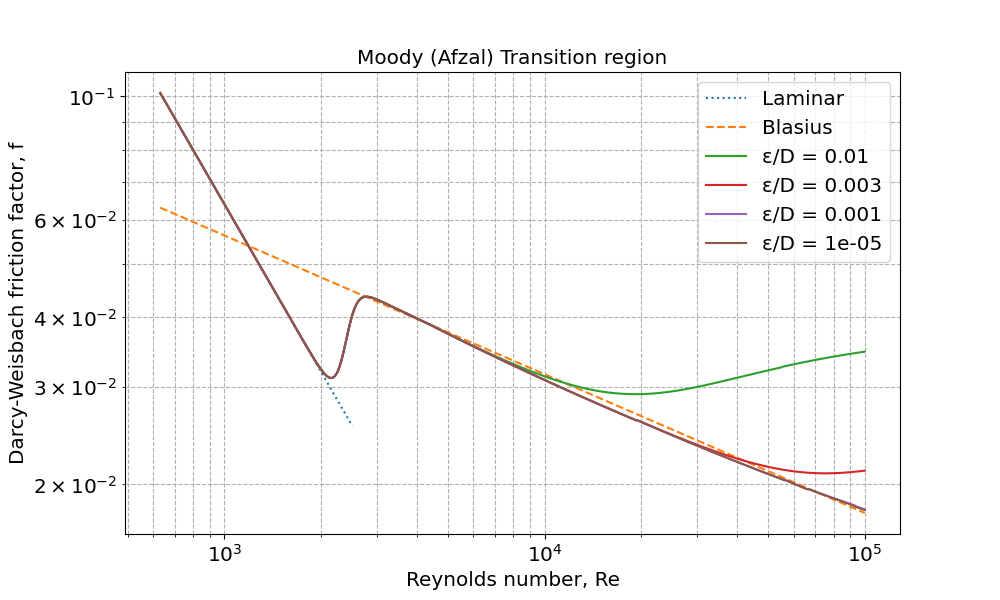
\includegraphics[width=0.49\textwidth]{moody_afzal_enlarge.png}
\caption{Darcy-Weisbach friction factor - Modified Afzal }
\label{fig:afzal-mod}
\end{figure}

We use the Azfal equation as the basis for our Moody plot and Pressure drop ratio figures by making the following additions:

\begin{enumerate}
    \item Where the Afzal line crosses the Blasius line, the modified Afzal is merged into the Blasius line over a range of Reynolds' numbers by taking the geometric mean of the two lines.
    \item Over the transition range to laminar behaviour, the modified-Afzal (now Blasius) line is merged into the laminar relationship with a logistic smoothing function.
\end{enumerate}

This gives a computationally smooth line which can be numerically differentiated and where the ratio of a hydrogen to natural gas lines can be computed without numerical artefacts. However the shape over the laminar-turbulent transition is only approximate and this version of the function has not been fitted to experimental data.

\section{Darcy-Weisbach Reynolds-Blasius material parameter}
\label{blasius2}
See Figure~\ref{fig:blasiusparam} to see that the Darcy-Weisbach Reynolds-Blasius material parameter 'B' (when normalised by the values for natural gas) varies by less than 1.2\% over the temperature range.
\begin{figure}[ht]
\centering
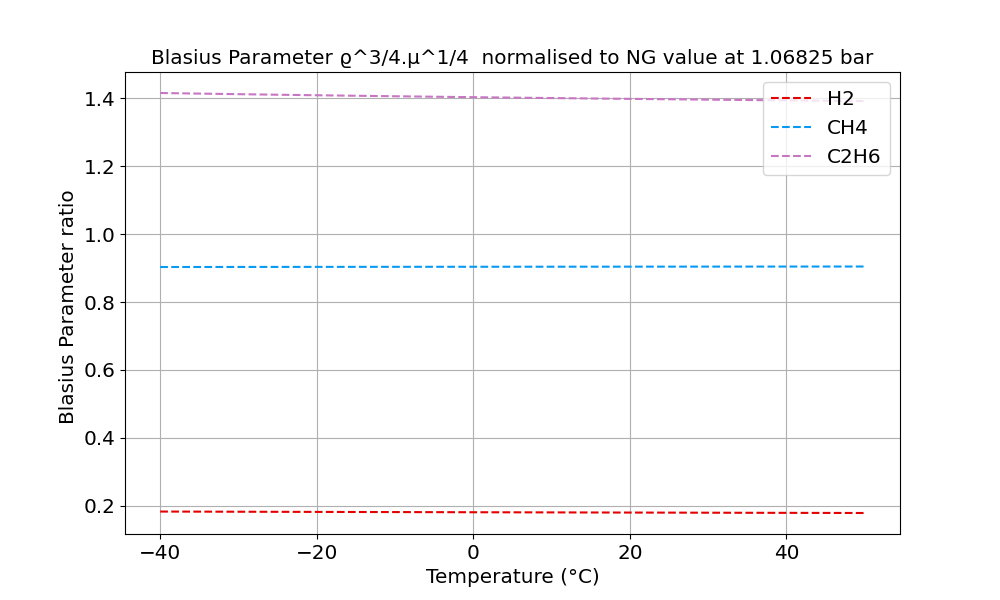
\includegraphics[width=0.49\textwidth]{peng_bf_NG.png}
\caption{Ratio of Darcy-Weisbach-Reynolds-Blasius material parameter  to that of natural gas NG }
\label{fig:blasiusparam}
\end{figure}
However, when considering pressures of 4 and 7 bar (5 and 8 bar absolute), the assumption of nearly-ideal behaviour does not hold. The properties of the gas are not nearly linear, so one can not assume that the behaviour along a pipe can be treated as a simple average of the behaviour at each end.



Blasius Parameter $\rho^{3/4}\mu^{1/4}$ normalised by the value for natural gas (Table~\ref{tab:Fordoun}) between -40.0$^\circ$C and 50.0$^\circ$C

\begin{figure}[htb]
\centering
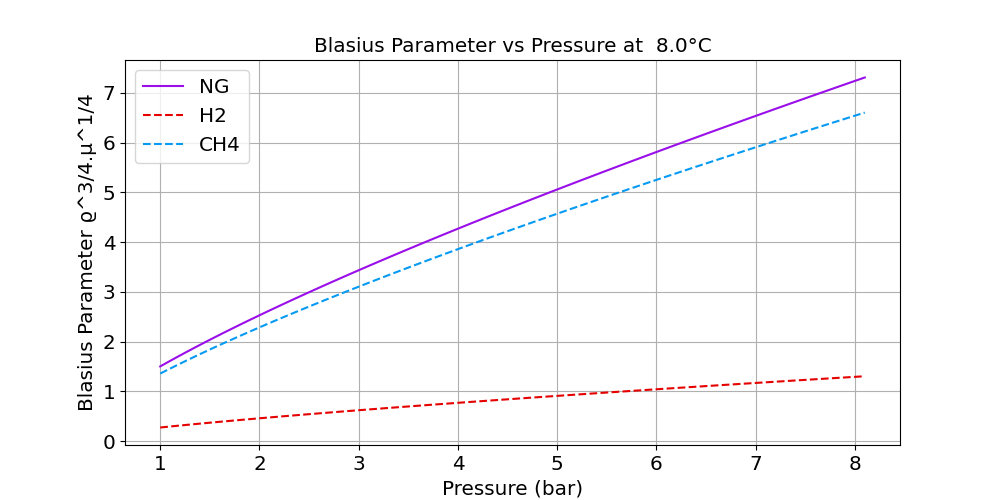
\includegraphics[width=0.49\textwidth]{peng_bf_p.png}
\caption{Darcy-Weisbach-Reynolds-Blasius material parameter depends on pressure }
\label{fig:blasiuspressure}
\end{figure}

\begin{table}[htb]
\begin{tabular}{r|r|l |l}
\hline
     1.06825 bar \\
\hline
H2       &0.1813 &$\pm$    0.0021&$\pm$   1.18\%\\
CH4      &0.9038 &$\pm$   0.0007&$\pm$  0.08\%\\
C2H6     &1.4032 &$\pm$    0.0119&$\pm$    0.85\%\\
\hline
     5.01325 bar \\
\hline
H2       &0.1794 &$\pm$ 0.0013  &$\pm$ 0.71\%\\
CH4      &0.9035 &$\pm$ 0.0009  &$\pm$ 0.10\%\\
C2H6     &1.4427 &$\pm$ 0.0300 &$\pm$  2.08\%\\
\hline
     8.01325 bar \\
\hline
H2       &0.1779 &$\pm$ 0.0006 &$\pm$  0.35\%\\
CH4      &0.9032 &$\pm$ 0.0010 &$\pm$  0.12\%\\
C2H6     &1.4801 &$\pm$ 0.0499  &$\pm$ 3.37\%\\
\end{tabular}
\caption{\label{tab:bparameter}Normalised 'B' Materials parameter gas/NG (-40.0$^\circ$C to 50.0$^\circ$C) showing temperature independence\citep{Sargents_github}}
\end{table}

\section{Flow at the turbulent transition}
\subsection{Hydrogen and Natural Gas comparative behaviour}
\label{h2ng}
If we look at how the friction factor changes when natural gas is replaced by hydrogen we get the family of curves in Figure~\ref{fig:h2ng}.

\begin{figure}[htb]
\centering
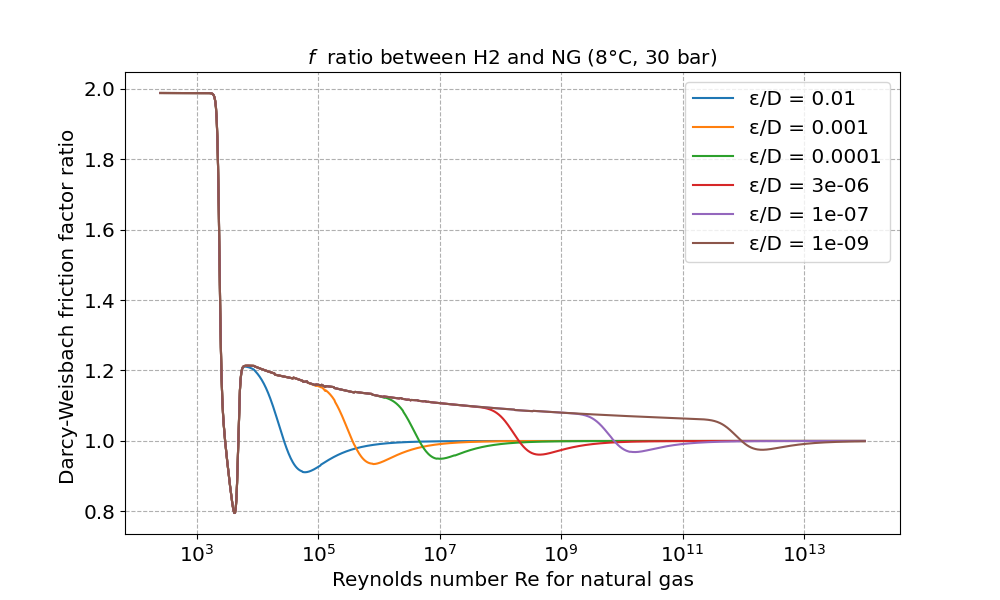
\includegraphics[width=0.49\textwidth]{h2_ratio.png}
\caption{Factor increase in Friction factor f  when natural gas is replaced with hydrogen with a velocity ratio of 3.076 .}
\label{fig:h2ng}
\end{figure}
When the velocity increases by a factor of 3.076 the Reynolds number decreases by a factor of 0.4103, at the pressure and temperature of the distribution service pipe.

When the flow is so low that both gases are in the laminar regime then the ratio of friction fractor is a steady2.4$\times$ higher for hydrogen than for natural gas. At large Reynolds' number, the increase in friction factor is zero because in that regime the flow is not sensitive to Reynolds' number at all. This is the case for smooth pipe above Re = 2.10$^9$

We find the ratio of the pressure drops for hydrogen and natural gas by taking the ratio of the two cases using equation \eqref{eqn:darcywiesbach}, copied here as equation \eqref{eqn:darcywiesbach2}.

\begin{equation}
\label{eqn:darcywiesbach2}
\Delta p = f \left( \frac{L}{D} \right) \frac{1}{2} \rho v^2
\end{equation}
where $L$ is the length of the pipe,  $D$ the diameter of the pipe,  $v$ is the mean velocity of the gas, $\rho$ the density, and $f$ the Darcy friction factor

\begin{equation}
\label{eqn:pdropratioturb2}
    \left(\frac{\Delta P_{H_2}}{\Delta P_{NG}}\right) = 
    \left(\frac{f_{H_2}}{f_{NG}}\right)
    \left(\frac{\rho_{H_2}}{\rho_{NG}}\right)
    \left(\frac{v_{H_2}}{v_{NG}}\right)^{2} 
\end{equation}

The terms in the ratios of $\rho$ and v do not change as Reynolds' number changes, so the required pressure drop to produce the same energy delivery as for natural gas is a curve of the same form.


\begin{equation}
\label{eqn:pdropratioturb3}
    \left(\frac{\Delta P_{H_2}}{\Delta P_{NG}}\right) = 
    \left(\frac{f_{H_2}}{f_{NG}}\right)
    \cdot
    1.03512
\end{equation}


\begin{figure}[htb]
\centering
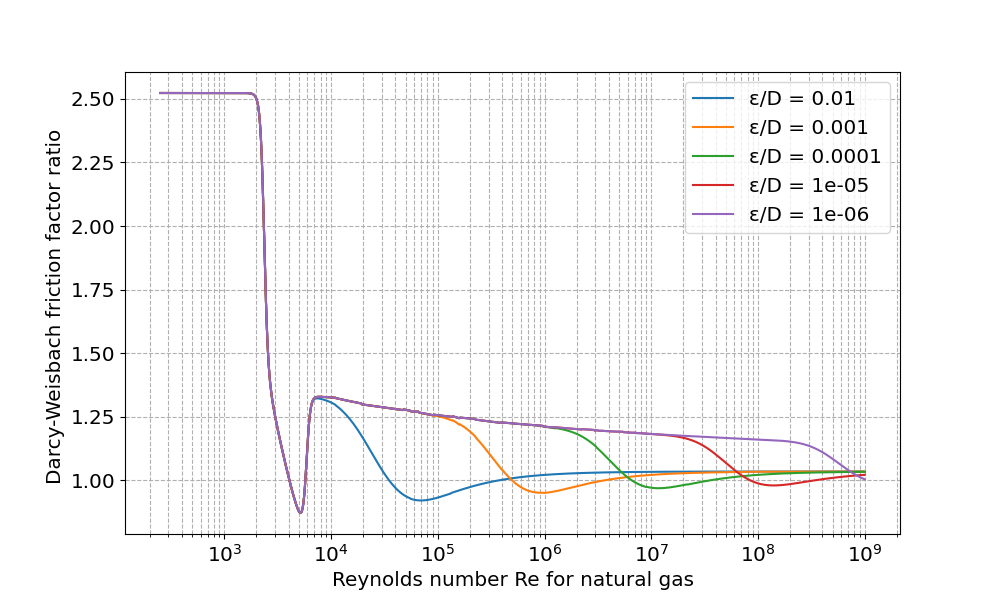
\includegraphics[width=0.49\textwidth]{p2_h2_ratio.png}
\caption{$\frac{\Delta P_{H_2}}{\Delta P_{NG}}$ \% increase when natural gas is replaced with hydrogen with a velocity ratio of 3.076 and a density ratio of 0.1094 .}
\label{fig:p2_h2ng}
\end{figure}

On reflection, one might wonder why the curve in Figure~\ref{fig:p2_h2ng} has only one minimum, whereas each of the natural gas and hydrogen friction factor curves have their own minima. The resolution of this can be seen in Figure~\ref{fig:h2ng_enlarge} where the double minima contributions can be seen in the shape of the single minimum. 

\begin{figure}[htb]
\centering
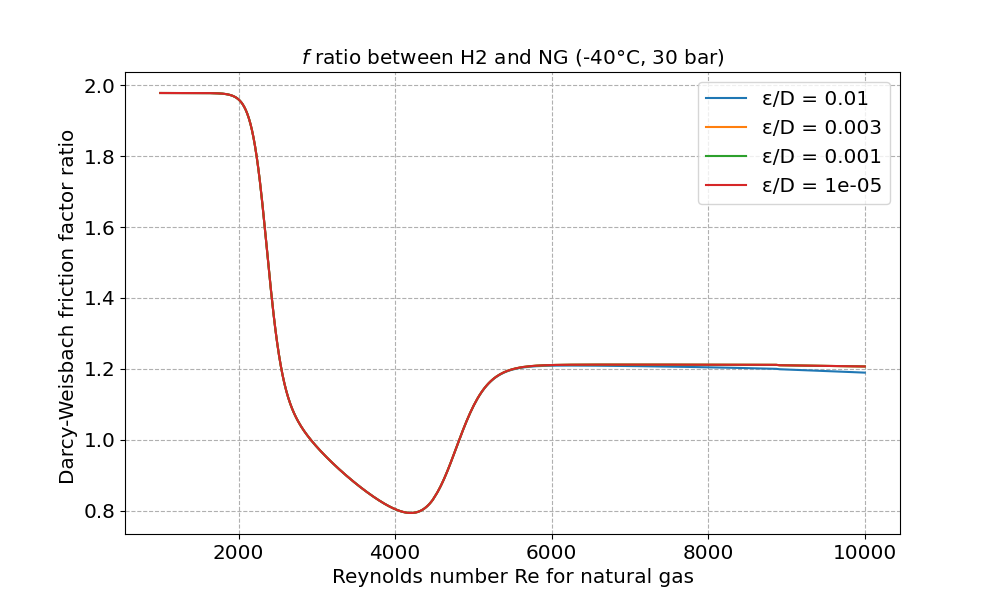
\includegraphics[width=0.49\textwidth]{h2_ratio_enlarge_lin.png}
\caption{Friction factor multiplier when natural gas is replaced with hydrogen on a linear-linear plot with a velocity ratio of 3.076. All curves for different roughnesses collapse to the same curve.}
\label{fig:h2ng_enlarge}
\end{figure}

\subsection{Gioia and Chakraborty}
\label{gioia}

Equation~\eqref{eqn:pdropratioturb2} is generically true for all flow regimes where the Darcy-Weisbach relation holds. So it is not valid for higher pressure gases where the behaviour along the pipe is not linear because of pressure effects.

Equation~\eqref{eqn:gcff} Relates the friction factor (f) to the Reynolds number (Re) and the roughness parameter (r)\citep{Gioia2006}. (Note that this is the Fanning friction factor, equal to four times the Darcy-Weisbach friction factor). It is shown in Figure~\ref{fig:gioia}.
\begin{equation}
\label{eqn:gcff}
f = \frac{0.8}{\left(Re/A \right)^{\frac{1}{3}}} \left( 1 + \frac{12}{\left(Re/B \right)^2} \right)^{-\frac{1}{2}}
\end{equation}

where the coefficients A and B are defined by \eqref{eqn:gcff-coeffs} in terms of the roughness ratio r=$\epsilon$/D:
\begin{equation}
\label{eqn:gcff-coeffs}
\begin{split}
A & = 30 + 8.8 r + 7.1 r^2 + 2.4 r^3 \\
B & = 550 + 33 r^2
\end{split}
\end{equation}


\begin{figure}[ht]
\centering
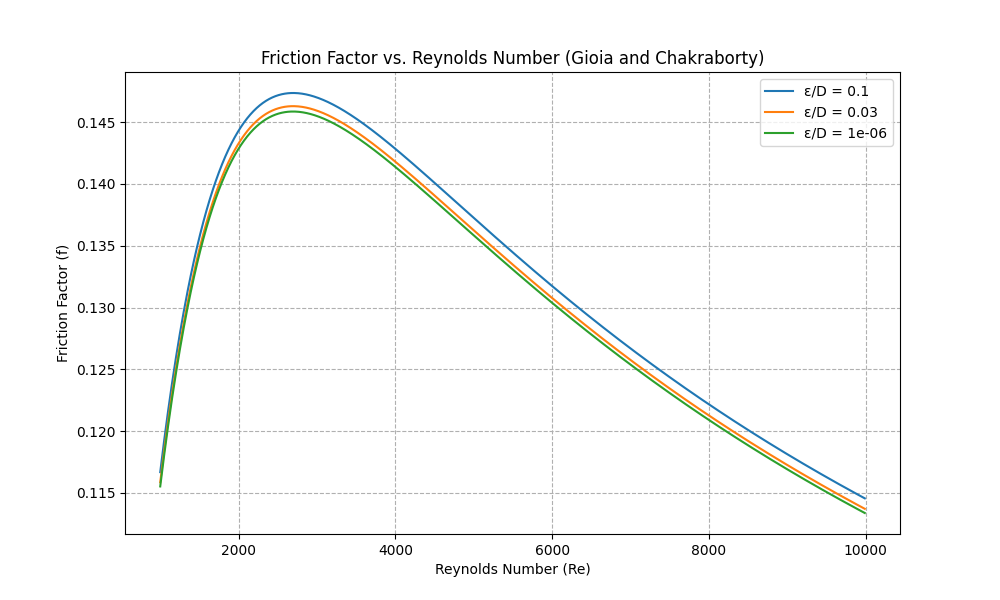
\includegraphics[width=0.49\textwidth]{gcff.png}
\caption{Friction factor for all pipe roughnesses at the turbulent transition.}
\label{fig:gioia}
\end{figure}

However  Brackbill has shown that the critical Reynolds' number is roughness dependent (Figure 9 in\citep{Brackbill2007}) and since 2018 it is now known that this is due to the time-average of laminar, slug and flash flow~\cite{Cerbus2018}.

The Colebrook equation \eqref{eqn:colebrook} does not represent the nikuradse 'hump' and 'belly' which recent research at Princeton and Okinawa shows is real.

\begin{equation}
\label{eqn:colebrook}
\frac{1}{\sqrt{f}} = -2.0 \log_{10} \left( \frac{(\epsilon/D)}{3.71} + \frac{2.51}{Re\sqrt{f}} \right)
\end{equation}

The Goldenfeld equation \eqref{eqn:goldenfeld} illustrates the form that any physically reasonable model should conform to~\cite{Goldenfeld2006}.

\begin{equation}
\label{eqn:goldenfeld}
f =   Re^{1/4} \cdot  g \left( Re^{3/4}, \epsilon/D  \right )
\end{equation}

It should be observed that none of the semi-empirical curve fits of Colebrook, Afzal, Swarmee etc. conform.
\begin{quote}
``The nikuradse
data show four features: a hump, the Blasius regime, a
shallow minimum, and the Strickler regime. The scaling
argument presented here implies that the Blasius and
Strickler regimes are both manifestations of inertial range
scaling coupled with wall friction, and, indeed, Gioia and
Chakraborty\citep{Gioia2006} find from momentum flux considerations that
this is sufficient to reproduce the Blasius and Strickler
regimes."~\cite{Goldenfeld2006}
\end{quote}

\section{Piping design rules}
\label{sec:pipe-rules}

The design rules\citep{GPS2008} for expected pressure drop along polythene pipe have a power law exponent of 1.17. This matches none of the theories referenced in this paper.
\begin{figure}[ht]
\centering
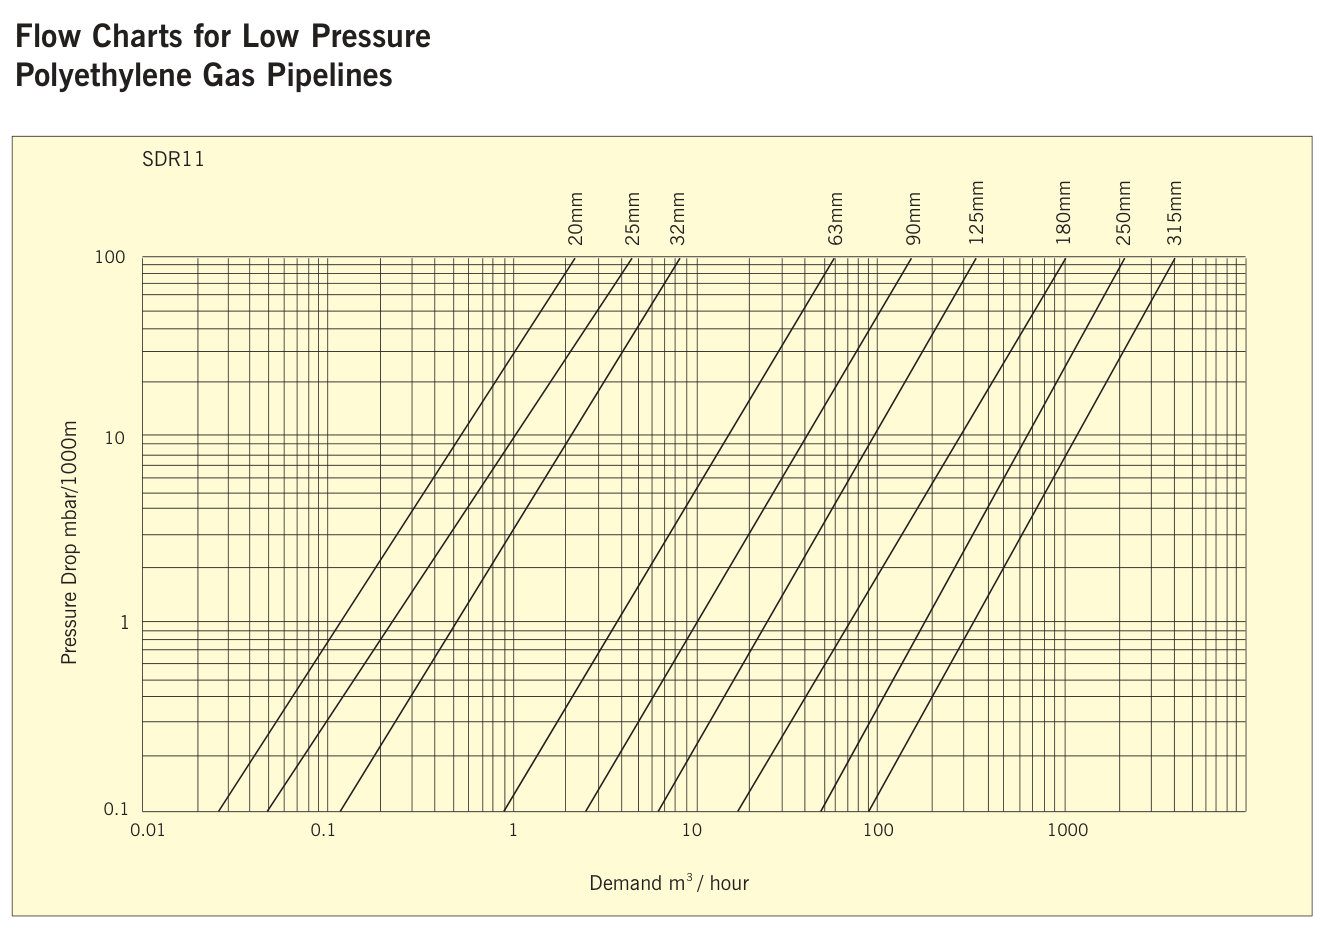
\includegraphics[width=0.49\textwidth]{sdr11-design-rules.png}
\caption{Design rules for specifying PE gas pipelines}
\label{fig:pipe-rules}
\end{figure}

The dimensions of the pipe are the outside diameters. The SDR11 specification is that a 32mm OD pipe has an internal bore of 25.8mm.


\section{Modelling Background} 
High-level economic models of hydrogen deployment use quite different, less detailed calculations for how hydrogen flows in an existing network than do detailed engineering designs.

These broad-brush models can unwittingly promote inaccurate intuitions which are not mere matters of detail. While it is true that pure hydrogen requires a volumetric flow rate nearly 3$\times$  that of natural gas to provide the same combustion power, it is not true that this requires pipelines 3$\times$  the size, or running an existing pipeline at 3$\times$  the pressure.

A techno-economic model needs simple formulae to describe technology choices. Unfortunately the voluminous technical literature on the delivery of hydrogen through pipes does not always present the results in a form that can be used, or even understood, by techno-economic modellers. 

\subsection{Policy making}
Techno-economic models need to evaluate required equipment capability at peak demand as this determines the capital expenditure. They also need to calculate the mean throughput over each year as this determines the running costs, e.g. the annual energy requirement for pumping hydrogen. But rather than central values for each of these, a policy-relevant model would produce upper and lower bounds. This means that upper and lower bounds on the friction values of hydrogen flows are useful, even if (as is the case) the actual turbulent behaviour is uncertain.

\end{document}


